%\documentclass[review]{elsarticle}
%\documentclass[preprint]{elsarticle}
%\documentclass[1p]{elsarticle}
%\documentclass[3p]{elsarticle}
%\documentclass[5p]{elsarticle}
\documentclass[final,5p,times,twocolumn]{elsarticle}
%\documentclass[final,5p,twocolumn]{elsarticle}

\usepackage[utf8]{inputenc} % Включаем поддержку UTF8
\usepackage[T2A]{fontenc}
\usepackage[russian,english]{babel}   % убрать русский перед отправкой статьи
\usepackage{lineno}
\usepackage{graphicx}
\usepackage{xcolor}
\usepackage[pdftex, backref, colorlinks]{hyperref}
\usepackage{multirow}
\usepackage{enumitem}


\graphicspath{{./figs/}}

\modulolinenumbers[5]
\journal{Astroparticle Physics}

%%%%%%%%%%%%%%%%%%%%%%%
%% Elsevier bibliography styles
%%
%% `Elsevier LaTeX' style
\bibliographystyle{elsarticle-num}
%%%%%%%%%%%%%%%%%%%%%%%
%\hyphenpenalty=10000
%\setlength{\marginparwidth}{2cm}
\usepackage{todonotes}

%http://ctan.math.washington.edu/tex-archive/macros/latex/contrib/easy-todo/easy-todo.pdf
%\usepackage[enable]{easy-todo}

\begin{document}
\newcommand{\todoi}[1]{\todo[inline]{ #1}}

\tableofcontents  % пусть пока побудет, стереть перед подачей
\listoftodos[Notes]
\linenumbers

\begin{frontmatter}
\title{SPHERE-2 balloon experiment results.\\ Part I: EAS observations conditions.}
%\todoi{Уточнить название статьи}
%\title{EAS observation from the air in the SPHERE-2 experiment. \\ Part 1. Atmosphere monitoring.

\author[address1]{E.A.~Bonvech\corref{correspondingauthor1}}
\cortext[correspondingauthor1]{Corresponding author}
\ead{bonvech@yandex.ru}
\author[address1]{D.V.~Chernov}
\author[address1]{T.A.~Dzhatdoev}
\author[address2,address3]{M.~Finger}
\author[address2,address3]{M.~Finger Jr.}
\author[address4]{V.I.~Galkin}
\author[address4,address1]{D.A.~Podgrudkov}
\author[address1]{T.M.~Roganova}
\author[address4,address1]{I.A.~Vaiman}
\address[address1]{M.V. Lomonosov Moscow State University, Skobeltsyn Institute of Nuclear Physics (SINP MSU), Moscow, Russia}
\address[address2]{Charles University, Faculty of Mathematics and Physics, Prague, Czech Republic}
\address[address3]{Joint Institute for Nuclear Research, Dubna, Russian Federation}
\address[address4]{M.V. Lomonosov Moscow State University, Department of Physics, Moscow, Russia}

\begin{abstract}
The SPHERE-2 detector designed for the extensive air showers detection was developed and performed measurements in 2011--2013. The data the detector collected is still under analysis but here we present the analysis of the telemetry data and of the detector operation conditions including temperature conditions and its effects, atmosphere studies.%\todoi{переписать под фактическое содержание статьи после завершения текста статьи.}
\end{abstract}

\begin{keyword}
primary cosmic rays\sep extensive air showers\sep Vavilov--Cherenkov radiation\sep balloon
\MSC[2010] 00-01\sep  99-00
\end{keyword}
\end{frontmatter}

\section{Introduction}
The SPHERE-2 experiment was designed for the primary cosmic ray (PCR) studies in the 10--1000~PeV energy range. The PCR particles induce the secondary particle cascades (extensive air showers, EAS) and secondary radiations (such as Cherenkov light, fluorescent light, radio emission) in the atmosphere that are registered by different methods by the ground-based detectors. However the SPHERE-2 experiment is a first successful implementation of a new EAS detection method --- detection of the reflected Cherenkov light (CL) using an aerial-based detector --- a method first proposed by E.~Chudakov~\cite{chu74:VKKL74} and pioneered by R.~Antonov~\cite{ant75, ant86, ant97, Ant15a}.

%The optical methods of EAS registration cannot compete with charged particles detectors (like KASCADE~\cite{}\todoi{Ссылка на KASCADE} or HAWC~\cite{}\todoi{Ссылка на HAWC}) in statistics due to very limited duty cycle. However, total CL flux from EAS has a very low dependence on the primary particle mass and hadron interactions model allowing for accurate energy estimation of every registered event with low systematic error. So the main goal of the SPHERE experiment is to measure as accurately and reliably as possible the PCR flux in given range. The small scale structure and features of the PCR energy spectrum are better studied with particle detectors albeit with not so good energy calibration.

Common EAS arrays such as the Telescope Array~\cite{abu12}, Yakutsk EAS array~\cite{Yakutsk19} or the TAIGA~\cite{TAIGA20} detector are the ground-based structures that are spread over up to hundreds~\cite{abu12} square kilometers. Significant effort is needed in order to install sensitive elements of such a vast arrays and to keep their network connected, power-supplied and time-synchronized. More effort is needed for the regular calibration of detector stations and for atmosphere parameter control over the detector area. 

On the other hand, conventional imaging air Cherenkov telescopes (IACT, like HESS~\cite{HESS03a, HESS03b} or MAGIC~\cite{MAGIC16-1, MAGIC16-2} are relatively compact systems that have good calibration means, high integrity power supply, atmosphere transparency control and so on. But since the Cherenkov light from EAS has a very narrow directional pattern it can not be observed by detectors more than about 0.5--1.5~km far from the shower axis. Therefore the IACTs have relatively low upper energy threshold.

The reflected CL method allows, on one hand, to register EAS on the relatively large area and later reconstruct the Cherenkov photons lateral distribution function, and, on the other hand, to utilize a small size compact detector with all the advantages of such setup. The mentioned advantages include (but are not limited to) the opportunity to implement: a complex topological trigger conditions prior to writing data to storage thus increasing the maximum operational count rate; direct on-line calibration system; high mobility with lower operational costs etc.

The compact detector that observes large surface area, however, can combine some strong sides of an IACT with high upper energy threshold. The main drawback of this design, however, is that a detector is significantly limited in its weight and therefore size. This means that detector's sensitive element should preferably operate in photon counting mode. This requires a good understanding of detector state and measuring conditions.

The general overview of the SPHERE-2 experiment can be found in~\cite{Ant15a}, and the detailed description of the detector electronics is given in~\cite{Ant20}. 

Here we present an overview of data registered by various auxiliary sensors on board of the SPHERE-2 detector. This data, collected during and in some cases before and after the EAS measurements, was used in the subsequent analysis for detector state and environment conditions control, allowing to perform various cross-checks of detector calibration, positioning and performance.



\section{The SPHERE-2 detector \label{sect:detector}}


The \mbox{SPHERE-2} is a compact detector designed to register the reflected Cherenkov light from EAS. The detector is lifted using tethered balloon to altitudes up to 1~km above the snow covered surface. Special tethered balloon BAPA~\cite{Ant20} was developed and manufactured by Russian Augur balloon systems agency~\cite{Augur}.

The \mbox{SPHERE-2} detector optics comprised a 1.5~m diameter spherical mirror with a 109 photomultiplier tubes (PMT) mosaic (optical scheme of the detector is shown in Fig.~\ref{fig:optics}).

\begin{figure}[bt]
\centering
    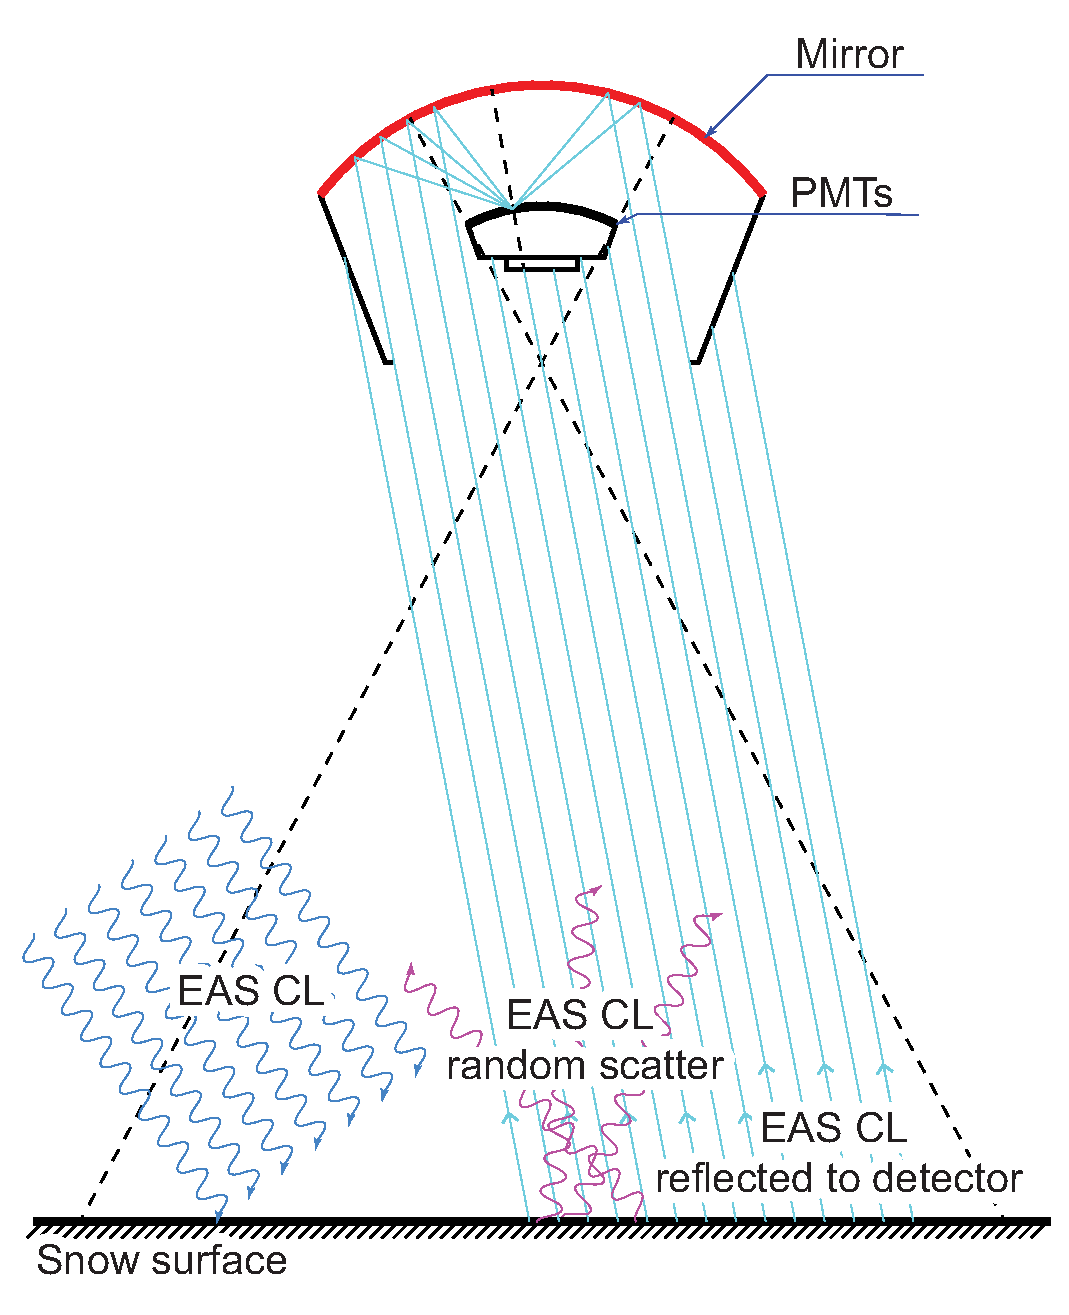
\includegraphics[width=0.42\textwidth]{optics}
    \caption{The detector optical scheme.}
\label{fig:optics}
\end{figure}

The PMT mosaic was located near the mirror focal surface and recorded light reflected from the snow surface below the detector. PMTs were arranged in the hexagonal structure on the spherical surface (see details in~\cite{Ant20}, or below on Fig.~\ref{fig:2012-3_shore_image}). The FEU-84/3 PMTs were used in the mosaic. The exact number of PMTs in each season are given in Tab.~\ref{tab:statistics}. The fields of view of PMTs are fixed in angular terms. The exact shape of the area that a single PMT observes depends on the PMT's position in the mosaic and the detector orientation.



\begin{table}[tb]
\centering
\caption{The annual statistics of the SPHERE experiment on Baikal Lake.
}
\label{tab:statistics}
\vspace{1pc}
\begin{tabular}{|c||c|c|c|r|r|}
\hline
year  & flights & PMT    & time, & triggers \\ 
      &         & number & hours & detected \\ 
\hline \hline
\multicolumn{5}{|c|}{test runs} \\
\hline
2008 & 1 &  20 &  1 &  6180 \\ 
2009 & 3 &  64 & 13 & 10312 \\ 
2010 & 6 &  96 & 30 &  1343 \\
\hline
\multicolumn{5}{|c|}{experiment runs} \\
\hline
2011 & 4 &  96 & 30 & 20571 \\
2012 & 5 & 108+1 & 31 &  7716 \\
2013 & 5 & 108+1 & 33 &  3813 \\
\hline
\end{tabular}
\end{table}

\subsection{Control block telemetry}
% кратко, что меряем служебного в блоке электроники: ЦАП и АЦП, какие токи, какие температуры, где температуры.
% кратко про мозаику

The control block of the SPHERE-2 detector contained a large array of different sensors along with the main registration electronics and power system. Sensors located both inside and outside of the control block were used to monitor detector state and performance, collect supplementary data for the EAS measurements. The list of the sensors used, their measuring range, precision and data collection frequency is given in table~\ref{tab:telemetry_sensors}. 

%%%%%%%%%%%%%%%%%%%%%%%%%%%%%%%%%%%%%%%%%%%%
%%% === Telemetry table === %%%
\begin{table*}[bth]
\centering
\caption{SPHERE-2 telemetry data readout intervals and sensors precision.}
\label{tab:telemetry_sensors}

%\vspace{1pc}
\begin{tabular}{|c|l|l|c|r@{\hspace{1mm}}c@{\hspace{1mm}}l|c|}
\hline
\multicolumn{1}{|c|}{interval} & \multicolumn{1}{c|}{parameter} & \multicolumn{1}{c|}{data}  & \multicolumn{1}{|c|}{accuracy} & \multicolumn{3}{c|}{range}  & \multicolumn{1}{c|}{units} \\
%\hline
\hline
\multirow{6}{*}{1 sec} & \multirow{3}{*}{Detector position} &GPS altitude & 2 (1)* &  -1500&--&18000  & m a.s.l.\\
                                                      \cline{3-8}
                         &                              & GPS position & 4 (2)** & &---&& m\\
                                                      \cline{3-8}
                       &                              & GPS time (PPS)& 1 & &---&& $\mu$s \\
                       \cline{2-8}
                       & \multirow{2}{*}{Detector orientation} & inclination angles (resolution) X,Y& 0.3 (0.02)&$-$25&--&25&deg (\\
                                                      \cline{3-8}
                       &                              & compass azimuth (resolution) Z &2.5 (0.5)&0&--&360&deg\\
                       \cline{2-8}
                       &Control block                 & inner temperature& 1.5 & $-40$&--&70 &deg,$^\circ$C\\
\hline
\multirow{7}{*}{1 min} & \multirow{2}{*}{PMT status} & anode current & 0.03 & 0&--&125 & $\mu$A\\
                                                      \cline{3-8}
                       &                              & mosaic temperature & 1.5 & $-40$&--&70 & deg,$^\circ$C\\
                       \cline{2-8}
                       & Power source                 & high voltage (HV1) & 0.1 & 0&--&250 & V\\
                       \cline{2-8}
                       & \multirow{2}{*}{Barometer}   & pressure & 5 & 750&--&1100 & hPa\\
                                                      \cline{3-8}
                       &                              & temperature& 2 & $-20$&--&60 &deg,$^\circ$C\\
                       \cline{2-8}
                       & Balloon barometer            & pressure   & 3 & 0&--&1000 & Pa\\
                       \cline{2-8}
                       & Battery (19V)                & voltage & 0.01 & 0&--&40 & V\\
                       \cline{2-8}
                       & Constant voltage (5V)        & voltage & 0.01 & 0&--&40 & V\\
\hline
\multirow{5}{*}{10 min} & \multirow{3}{*}{PMT status} & first dinode voltage & 0.06 & 0&--&250 & V\\
                                                      \cline{3-8}
                       &                              & PMT temperature & 0.1 & -30 &--&50 & deg,$^\circ$C\\
                                                      \cline{3-8}
                       &                              & supply voltage & 0.006 & 0&--&25 & V\\
                       \cline{2-8}
                       & Trigger                      & counting rate &1&0&--&4& Hz\\
                       \cline{2-8}
                       & FADC boards                  & voltage (1.2, 2.5, 2.8) & 0.001 & 0&--&4 & V\\
\hline
\end{tabular}

\vspace{1mm}

\footnotesize \raggedright 
\hspace{6.5 mm}* 2 m accuracy according to the manufacturer provided data, 1 m accuracy according to our own analysis (see in section~\ref{sect:orientation} )

\hspace{5 mm}** 4 m accuracy according to the manufacturer provided data, 2 m accuracy according to our own analysis (see in section~\ref{sect:orientation} )
\normalsize
\end{table*}

%%%%%%%%%%%%%%%%%%%%%%%%%%%%%%%%%%%%%%%%%%%%

The sensors inside the control block measured:
\begin{itemize}[nosep]
\item the temperature of the FADC boards (two sensors per board) for cooling system operation;
\item the voltage on the secondary power supply units for PMT mosaic power stabilization;
\item the voltage and current on the main power supply unit;
\item the overpressure and temperature inside the balloon.
\end{itemize}
The sensors outside the control block measured:
\begin{itemize}[nosep]
\item detector position (GPS-module);
\item local air pressure and temperature;
\item compass.
\end{itemize}
Additional sensors were installed on the PMTs in the mosaic and controlled
\begin{itemize}[nosep]
\item power supply voltage;
\item anode current;
\item temperature.
\end{itemize}

Some data provided by these sensors was used to monitor the flight conditions and detector status in real time. Also, all the data was stored and later was used in EAS parameters reconstruction and in detector performance evaluation.

\subsection{Orientation control system}
\label{sect:orientation}

The detector axis at the rest state is oriented vertically and detector observes the snow covered surface just under the detector. During the measurements the detector hang under the balloon and swung and rotated freely. The detector inclination is an important factor for the shower parameters reconstruction as it determine the overall geometry of the experiment. To control the position and rotation of the detector a dual-axis inclinometer and a digital compass were installed on the PMT mosaic control board. 

The digital compass measures the angle of the detector's orientation relative to the Earth's magnetic field with 2.5~degree precision.

The inclinometer measures two angles between it's internal orthogonal axes and the plane orthogonal to the gravity vector. The orientation of inclinometer axes respectively to detector mosaic axes was determined in the laboratory. After careful preparations the mosaic was set horizontally with precision better than $0.3^\circ$\todoi{Уточнить по фактическому состоянию! Чернов Д.В.} and the zero level of the inclinometer was measured. All detector inclination angles were calculated considering recovered zero level.

The type of inclinometer used allows fast angles measurements with low power consumption, but, contrary to the gyroscopic ones, it is affected by acceleration. As we will see in sec~\ref{sect:telemetrydata} during detector flights there was recorded only a signle instance of strong wind gusts at the end of the 2013-3 flight, and the balloon position was relatively stable in all other times. So we assumed that the registered inclination angles were unaffected by swinging.

The GPS sensor Garmin 16xHVS~\cite{GPS-module-specs}, located on the control unit was used to measure geographical coordinates and an elevation above sea level. 

The GPS manufacturer declared the absolute accuracy of 4~m in position measurements, and 2~m accuracy in the altitude determination. Our observations show than an accuracy of position detection by the GPS sensor differs for moving and stationary situations. 

The accuracy position determination of the GPS sensor in stationary state was calculated from GPS data at a time when the detector was stationary on the ice. Daily distributions of the detector position and altitude were plotted for 20 days in 2012 and 2013. The median sigma of these distributions is taken as the accuracy of the position and altitude measurements: 2~m and 1~m respectively.

However, the detector showed significant lag in altitude measurements during initial balloon climb and subsequent flight altitude changes. More details on the lag, its correction and influence on detector altitude determination are discussed in Sec.~\ref{sect:gps_correction}.

%%%% Какая есть телеметрия %%%%%

\subsection{Telemetry monitoring\label{sect:telemetry}}

During every experimental flight a lot of information about the detector status and the environmental parameters was recorded. The different telemetry data was received and checked every second, every minute and every 10 minutes. 

Every second the detector position and orientation was recorded. The GPS data (altitude, latitude and longitude), universal global time UTC, the angles of detector inclination, digital compass data and the control block inner temperature was monitored. The additional GPS and barometer were deployed on the control booth at ice level.

Every minute the PMT and the power status were monitored. Anode currents of each PMT, the PMT mosaic temperature and the temperature of the PMTs high voltage power source as well as the power supply voltage and DC voltage sources were recorded. Barometer sensors were polled every minute also.

Every ten minutes the detector logged the PMTs supply voltages, voltages at PTMS first and tenth dynodes, individual PMT temperatures. The measuring channel counting rates and voltage on the FADC boards were also recorded.

% done \todoi{Описать в два слова, зачем оно тут в таком количестве регистрировалось}
The PMTs power supply data were later used to control the optical modules operational stability. The registered discriminator triggering rate was used for discriminator thresholds selection in experimental flights. The deviation of the power consumption in FADC boards was used to monitor possible malfunctions in the detector electronics. The temperature sensors data was used for in-flight detector state and cooling system control.

\section{Experimental conditions}
%\section{Site and weather}
\label{sect:data}
 
The SPHERE experiment was carried out on the Baikal Lake during winters 2008--2013. The Baikal lake ice thickness reaches 40--60~cm in February and can hold heavy vehicles. The balloon launch pad was deployed on the lake surface around 700~m from the shore (near 51$^\circ$\,47'\,48''~N, 104$^\circ$\,23'\,19''~E).
%51.796923~N, 104.388663~E http://www.google.com/maps?q=51.796923,+104.388663

The \mbox{SPHERE-2} detector was lifted by the tethered balloon BAPA to altitudes up to 900~m above snow surface. The annual statistics of the experiment is given by the Tab.~\ref{tab:statistics}. The first two years were test ones. The detector configuration was improved from year to year. Thus the number of PMTs was increased from 96 to 109, the signal sampling rate was changed in 2012 from~40~MHz to 80~MHz.


%Unless otherwise specified, all illustrations in the paper are given for the \mbox{SPHERE-2} data of the winter 2013 run. All plots were made with Python Matplotlib plotting library.

%% Baikal snow photo %% fig:baikal_snow
\begin{figure}[tb]
\begin{center}
    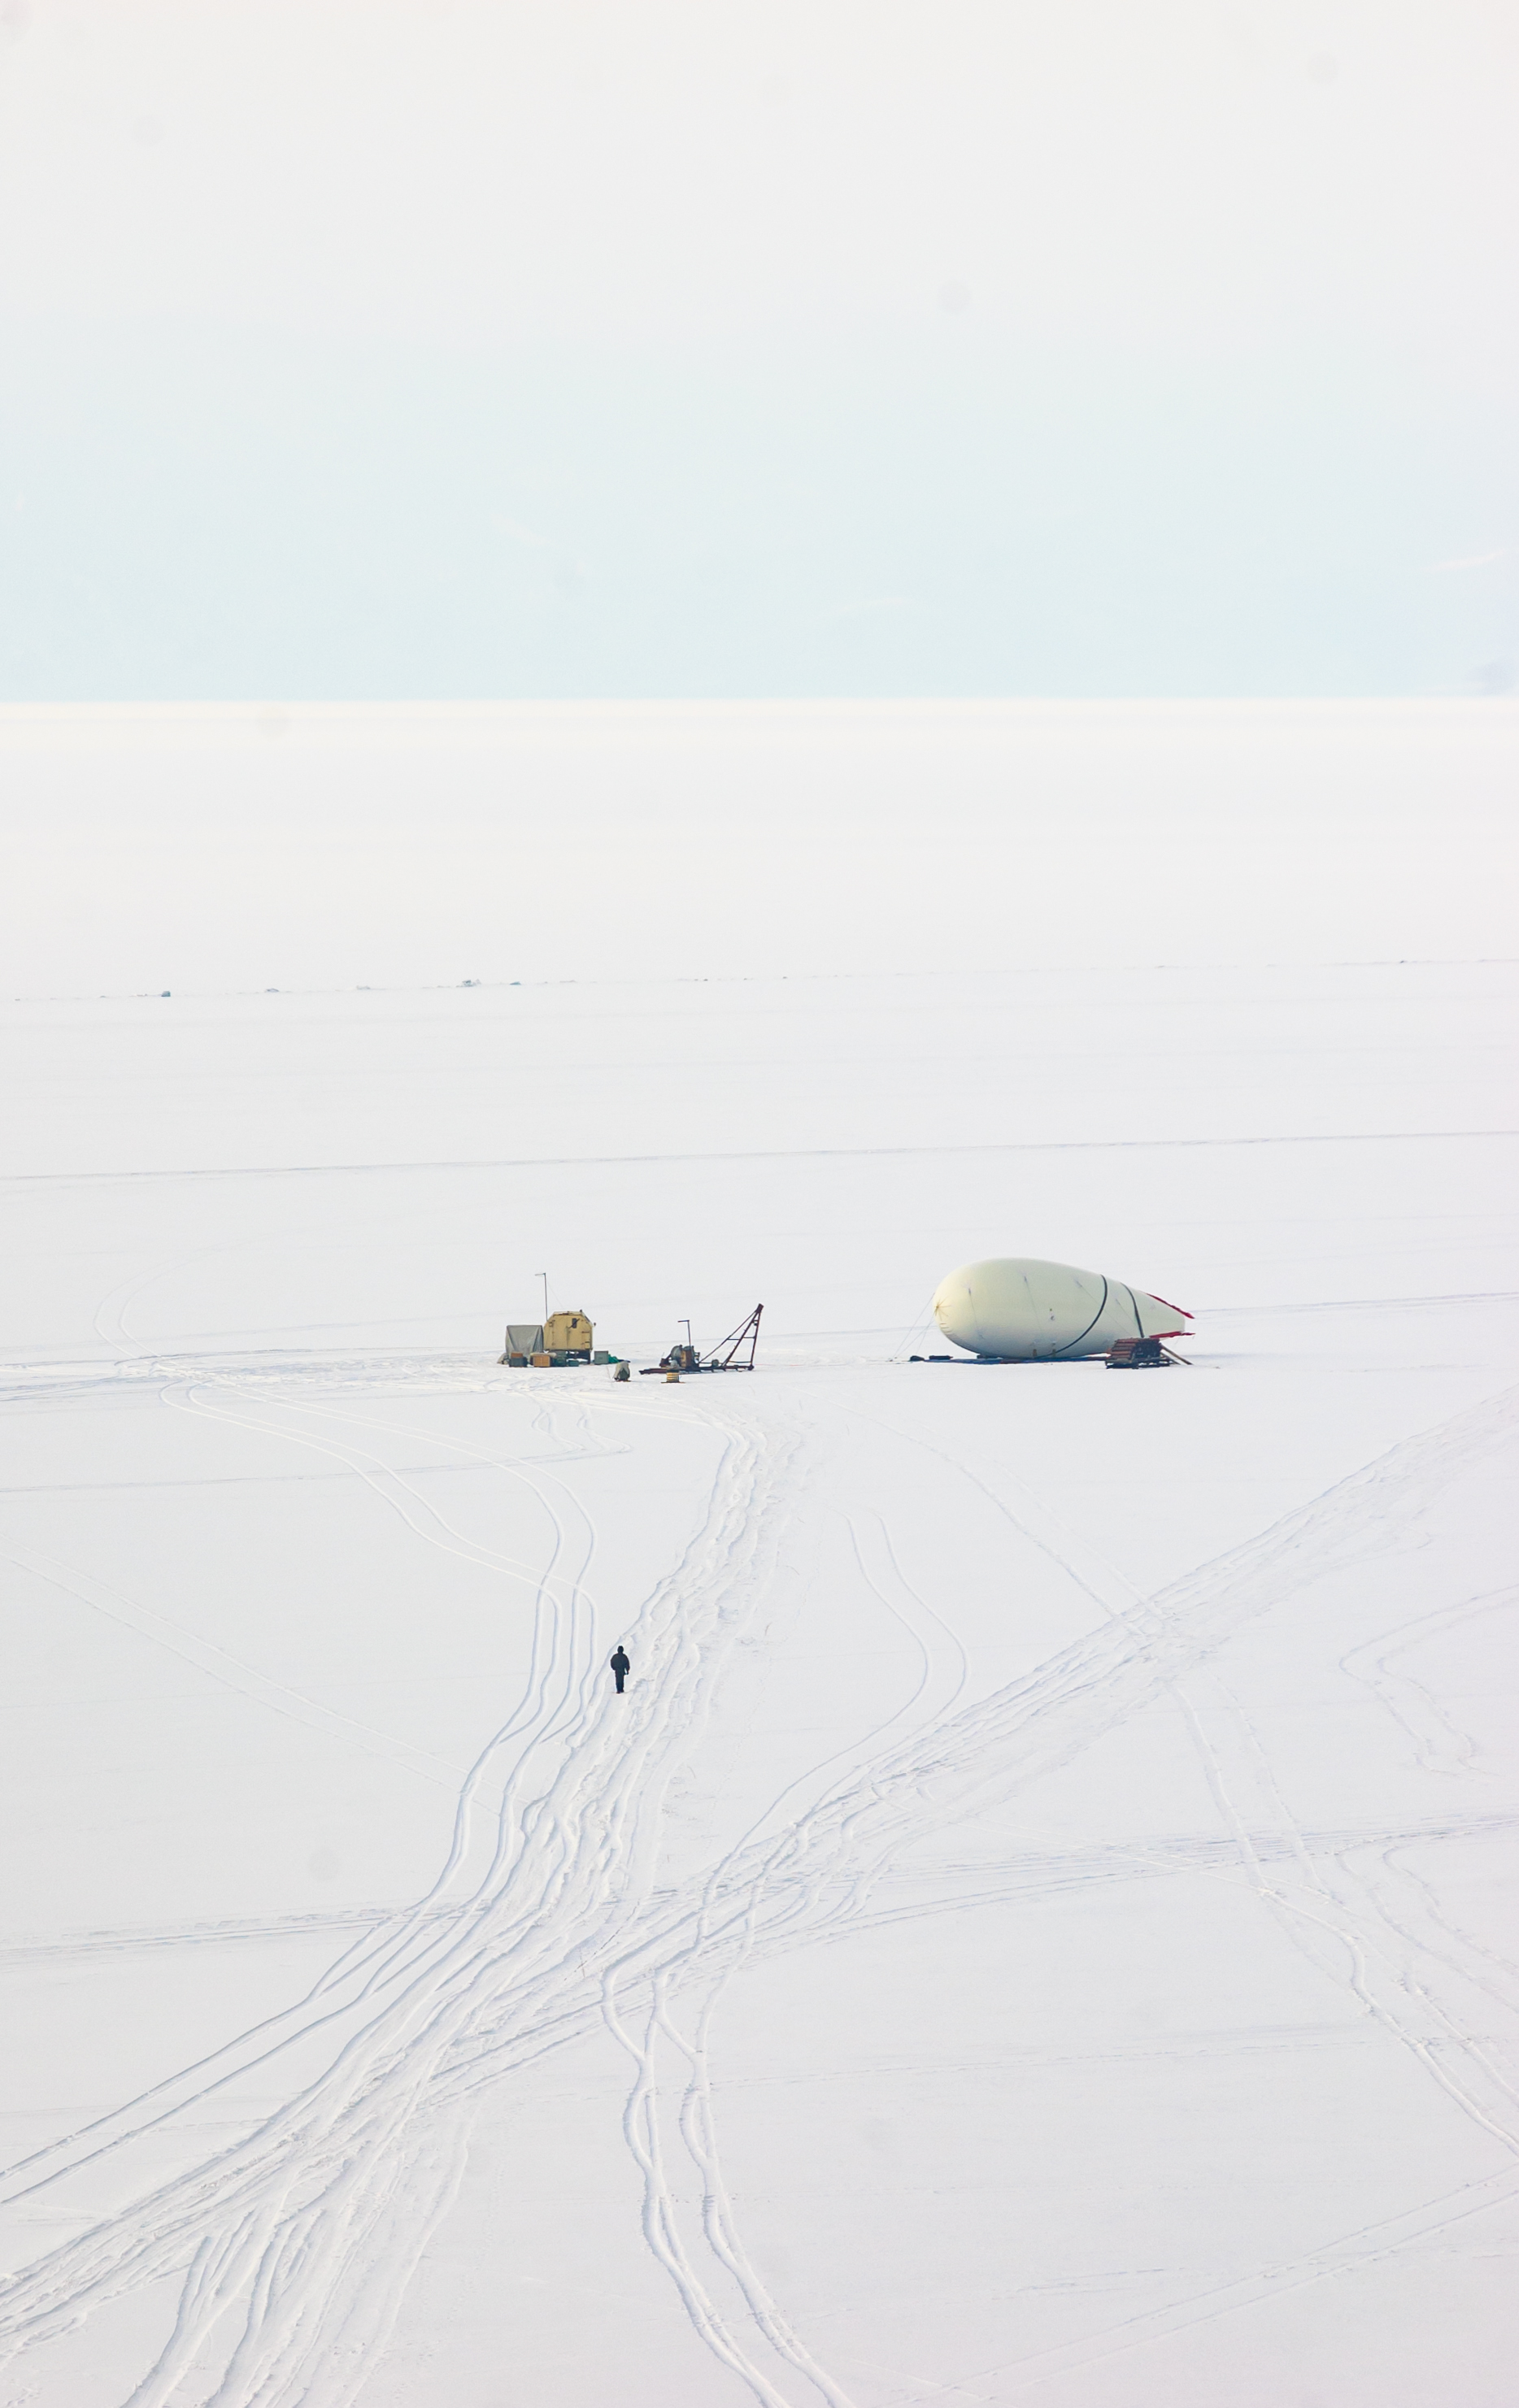
\includegraphics[trim=1cm 5cm 0cm 5cm,clip,width=0.45\textwidth]{DSC_4049.jpg}\hspace{2pc}%
    \caption{The overview of the launch site on the Baikal Lake from the hill on the shore. The snow coverage around the SPHERE start point was thick and was usually renewed between flights by occasional snowfalls.}
\label{fig:baikal_snow}
\end{center}
\end{figure}
\begin{figure}[tb]
\begin{center}
    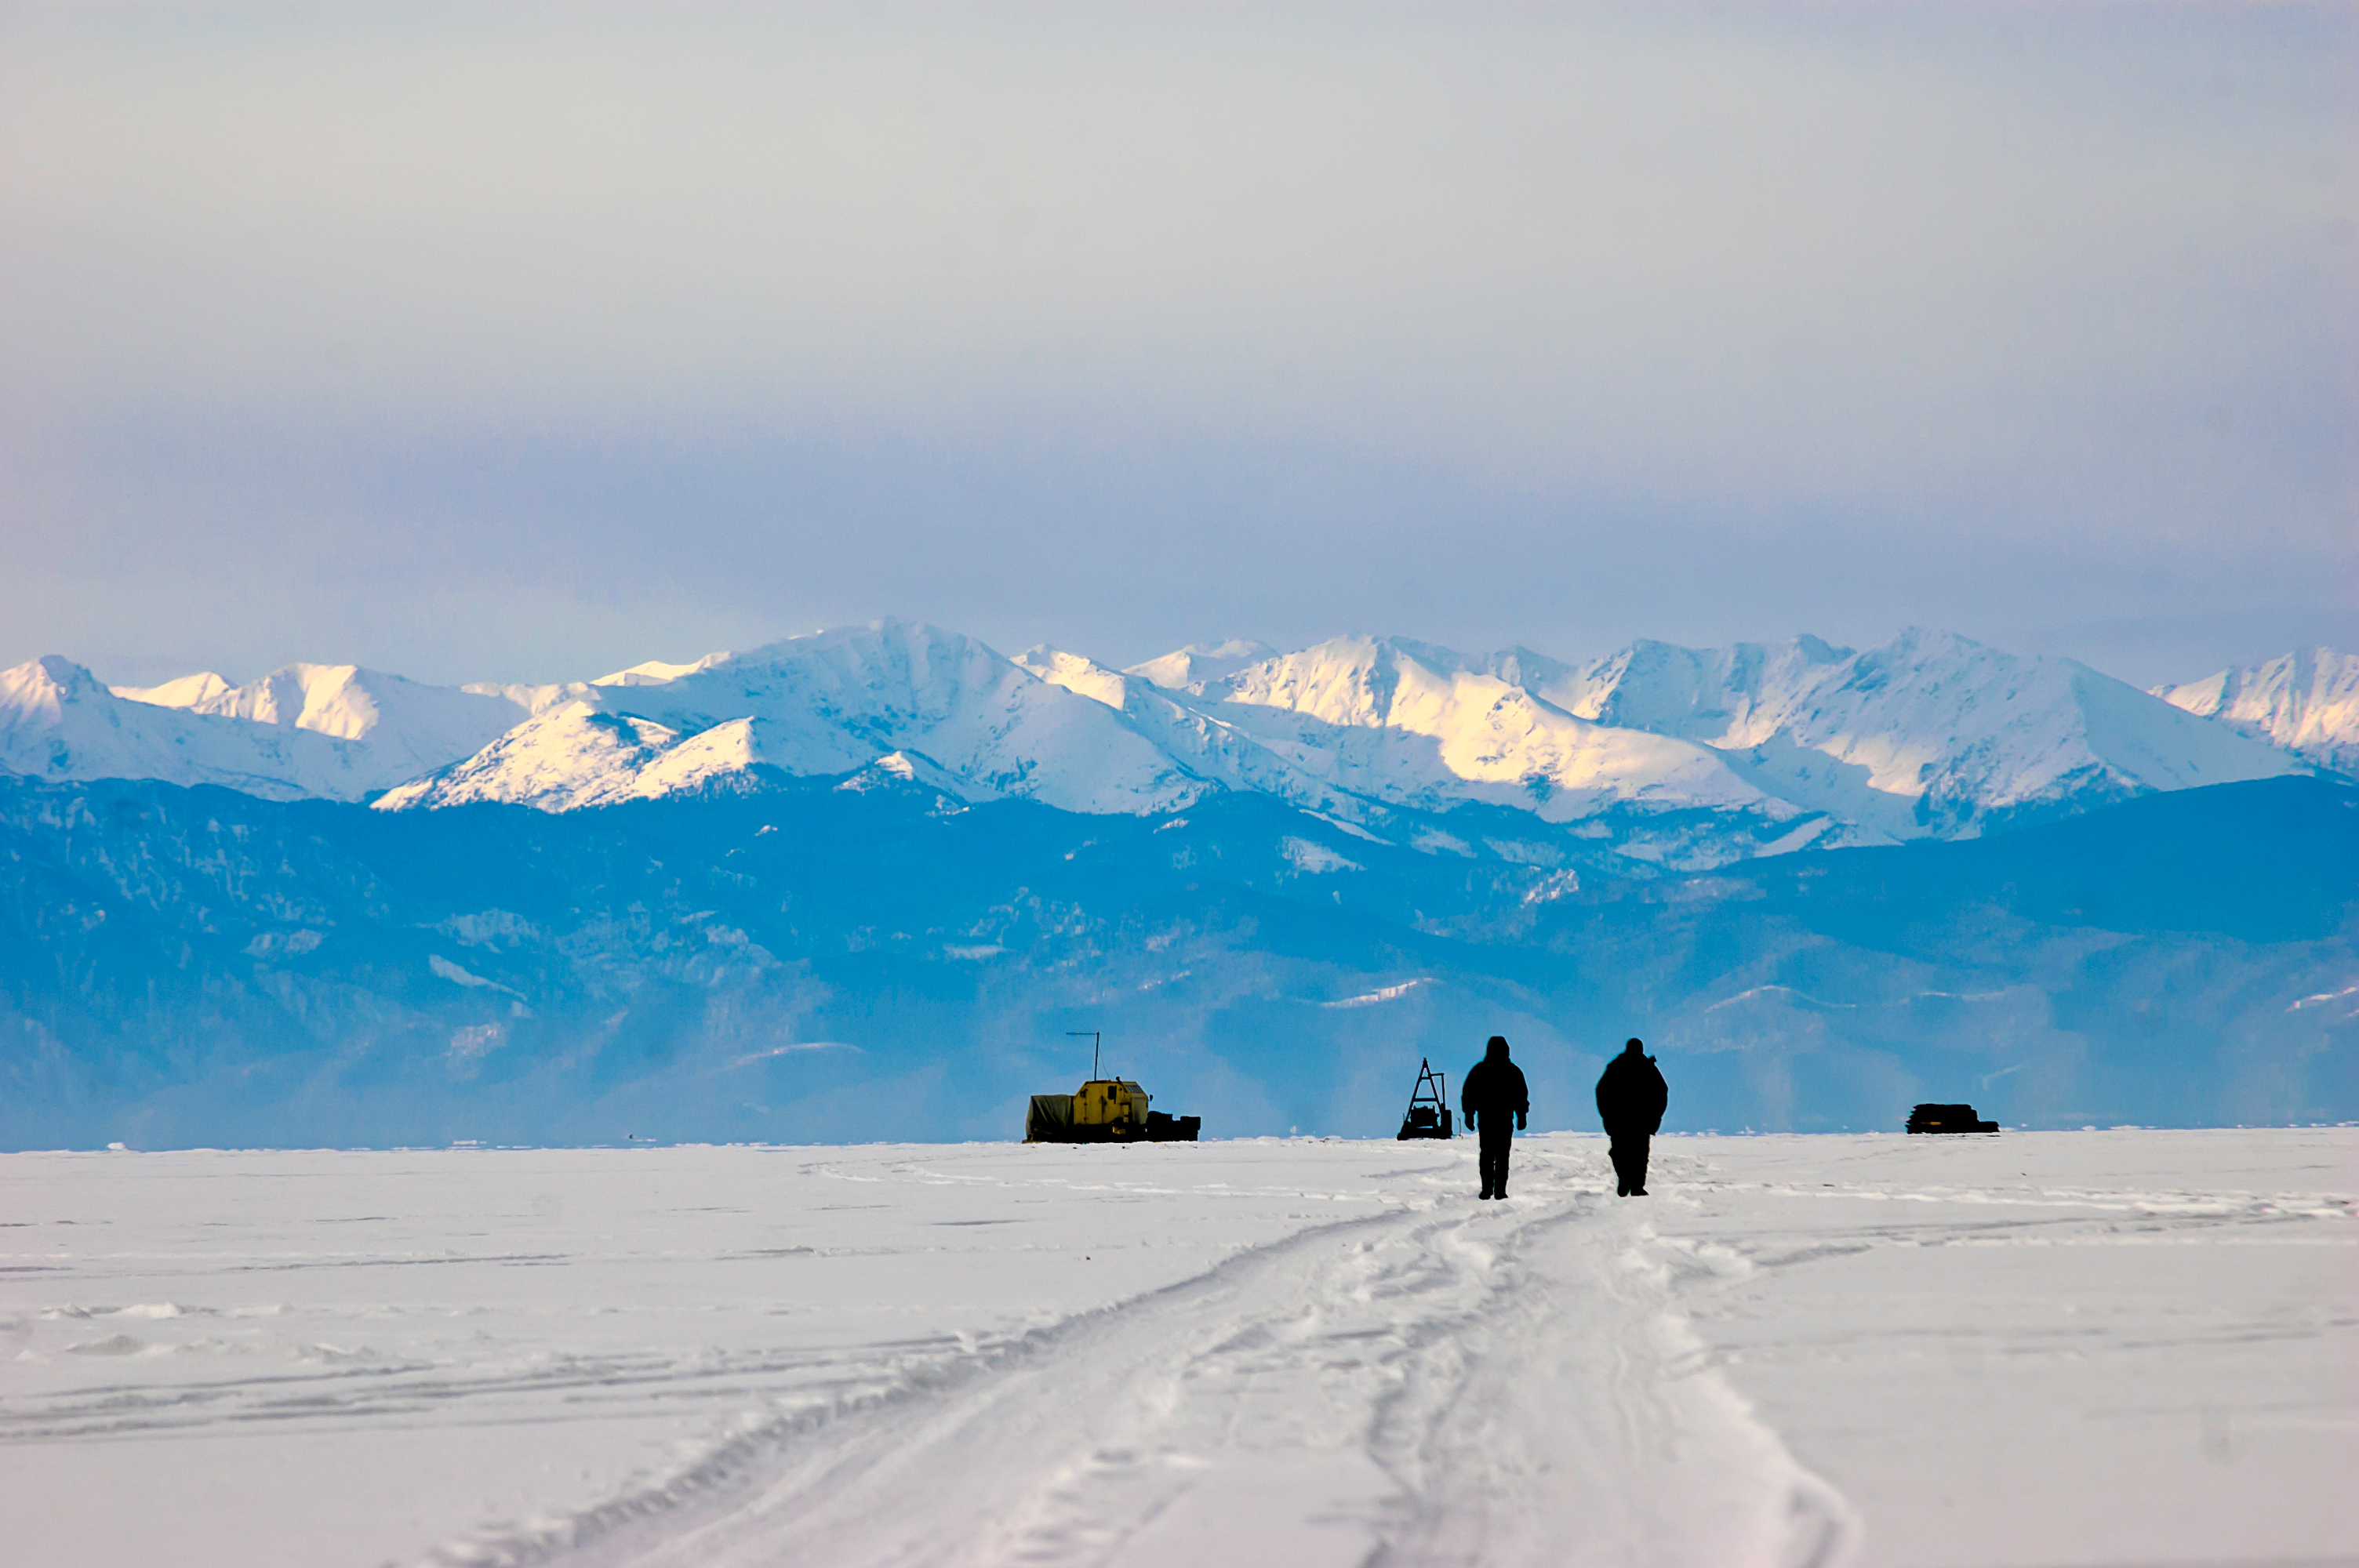
\includegraphics[width=0.45\textwidth]{DSC_7423.jpg}\hspace{2pc}%
    \caption{The overview of the launch site on the Baikal Lake from the shore. The background mountains are more than 50 kilometers away with indicates good atmosphere transparency on ground level.}
\label{fig:baikal_atmo}
\end{center}
\end{figure}

\subsection{Weather and snow}

Measurements were carried out during clear moonless nights with low wind. The measurements were started 1.5 hour after sunset or immediately after moon set and were finished before moon rise or 1.5 hour before sunrise. If the wind condition had become unsuitable for the flight the balloon with detector was landed at once (however, this happened only with the third flight in 2013). The typical night air temperature on the lake surface was near $-15^\circ$C. According to the \href{https://rp5.ru/Weather_in_the_world}{Reliable Prognosis} data archive~\cite{rp5} for the nearest weather stations 30818 and 30710 the horizontal visibility was `at least 10 km' (the highest possible grade in the system), and the altitude of the base of the lowest clouds was `2500~m or more or no clouds present'.

Our own observations of the atmosphere show that during the day the visibility degraded due to high humidity (as is the case show in Fig.~\ref{fig:baikal_snow}), but in the evening recovered back. In~Fig.~\ref{fig:baikal_atmo} the background mountains snow caps are 55--56~km away therefore the horizontal visibility was good. During nights the mountains were also visible. The Milky Way was clearly visible during all measurement nights. 

The measurements were performed in the end of winter season when Baikal lake was covered with thick ice. The snow coverage of the ice differed from year to year and in different areas of the lake according to prevailing winds. However in 2010--2013 winters the lake area near the launch site was covered thick (up to 40~cm) layer of snow with occasional snowfalls. In Fig.~\ref{fig:baikal_snow} the snow coverage in 2012 is shown. This was the typical coverage during measurements. The snow reflection properties were controlled using a photometer. The influence of the snow state on its reflecting properties has been discussed in detail in our article on the simulation of the SPHERE-2 detector~\cite{Ant19}.

Another atmosphere property that was monitored during measurements was its density. The optical transparency is a crucial property for Cherenkov-light-reliant methods of EAS studies since it directly influences measured light fluxes (and later the primary particle energy estimations). However, the atmosphere density profile is vital to the primary particle type studies since it affects the altitude of the shower development and its Cherenkov light lateral distribution function (CL LDF). The influence of the selected atmosphere on the CL LDF and its properties are discussed below in section~\ref{sect:atmosphere-profile}.

The atmosphere density profile was reconstructed based on the air pressure and temperature measurements during the initial climb in the beginning of the night and during descent at the end of the night. In almost all measurement nights the atmosphere remained stable. The stable atmosphere conditions were expected from the known Siberian High phenomena. However, in two flights 2012-3 and 2013-5 the rapid change in the atmosphere profile was observed (see Fig.~\ref{fig:density}) followed by the rapid weather worsening (clear sky changes to cloudy, wind became stronger with gusts), which, unfortunately, is indicative of the climate change and observed weakening of the Siberian High anticyclone. 

\subsection{Detector orientation and telemetry data}
\label{sect:telemetrydata}

The \mbox{SPHERE-2} detector's position and inclination depend on wind conditions near the detector (see. Fig.~\ref{fig:gps_compass} and Fig.~\ref{fig:inclination}). In Fig.~\ref{fig:gps_compass} the position of the detector with the magnetometer data is shown for some flights of the 2011--2013 seasons. The position was reconstructed using GPS data with launch point at zero coordinates. The detector orientation measured by magnetometer is indicated by arrows. Figure~\ref{fig:gps_compass} demonstrates that wind was quite constant during most of the time and the balloon position was rather stable and varied slowly.  

%%%%%%%%%%%%%%%%%%%%%%%%%%%%%
%% detector drift figure  %%%
%%% fig:gps-compass
\begin{figure}[tb]
    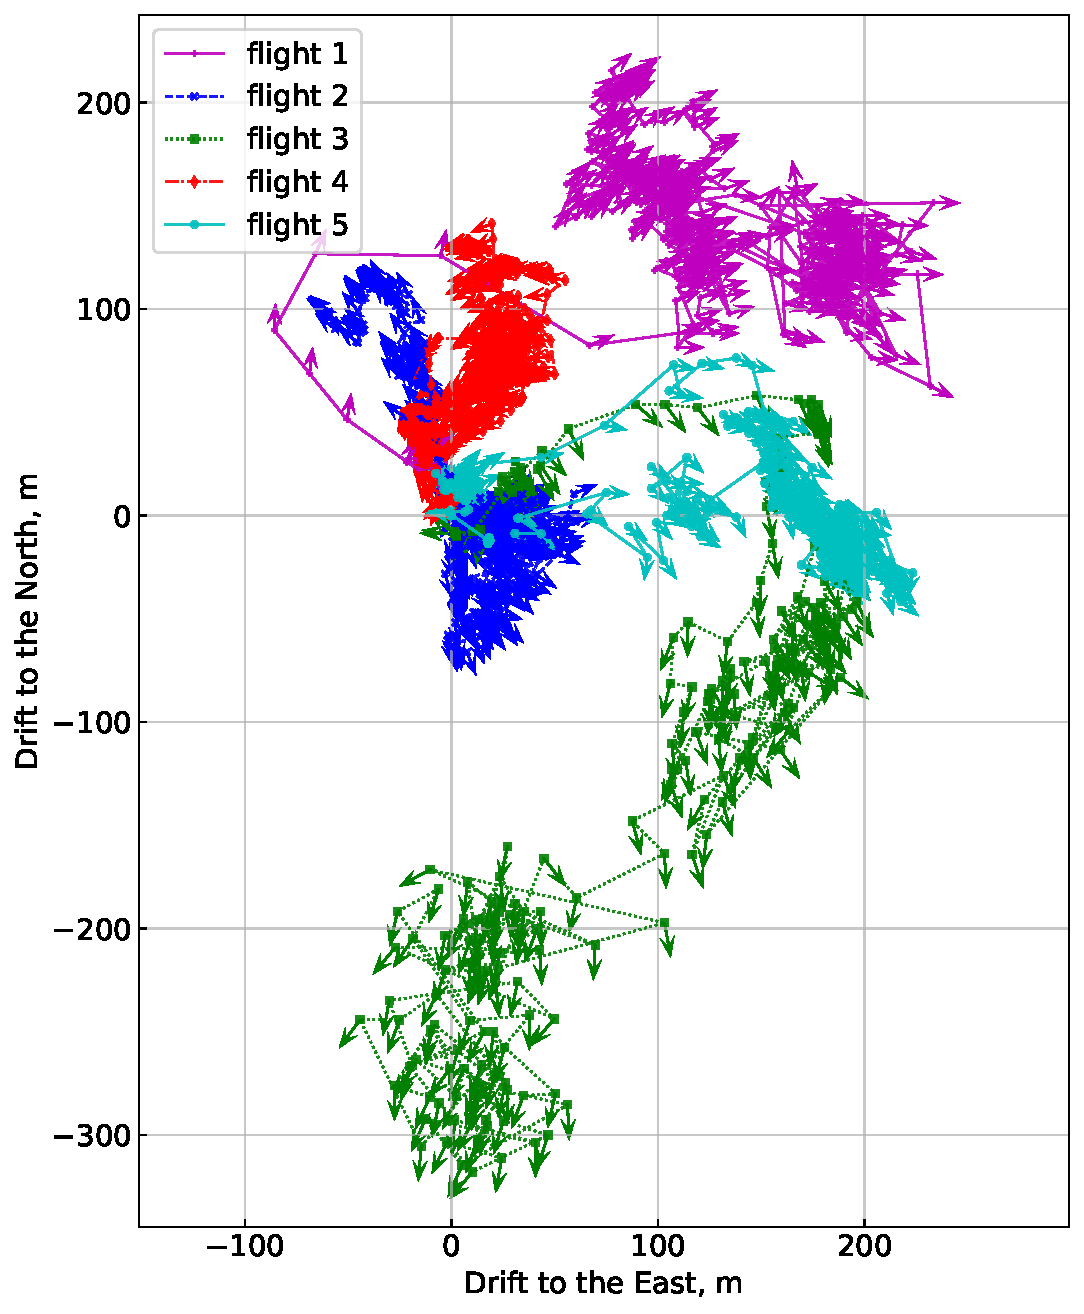
\includegraphics[width=0.45\textwidth]{GPS+quiver.pdf}\hspace{2pc}%
    \caption{The SPHERE-2 detector drift in 2013. The arrows indicate the detector magnetometer orientation. The start point is located at zero coordinates.}
\label{fig:gps_compass}
\end{figure}
%%%%%%%%%%%%%%%%%%%%%%%%%%%%%

%%%%%%%%%%%%%%%%%%%%%%%%%%%%%
%%  4 telemetry  pictures %%%
\begin{figure*}[tb]
    \begin{minipage}[t]{0.48\textwidth}
    \centering
    %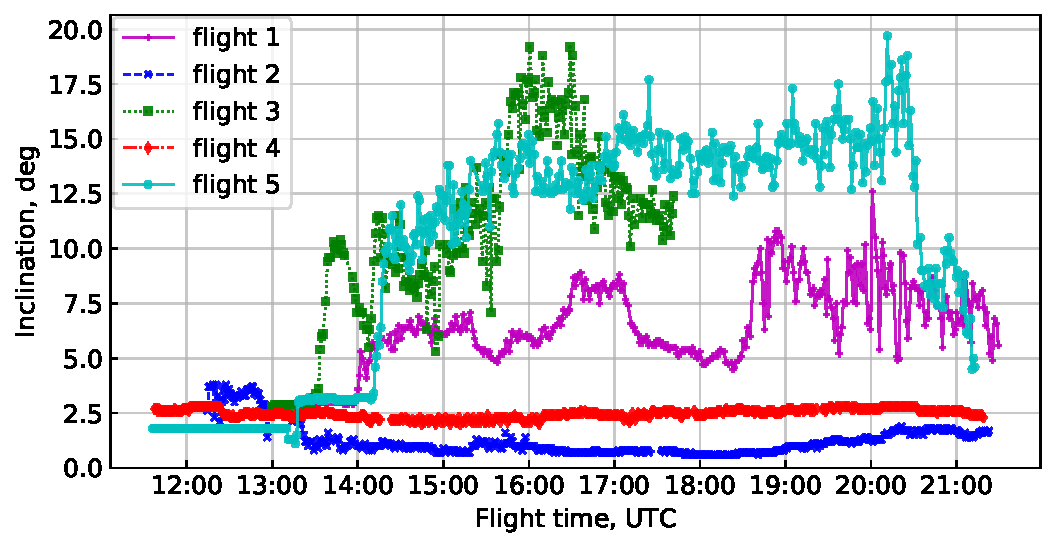
\includegraphics[width=\textwidth]{ClinTh.pdf}
       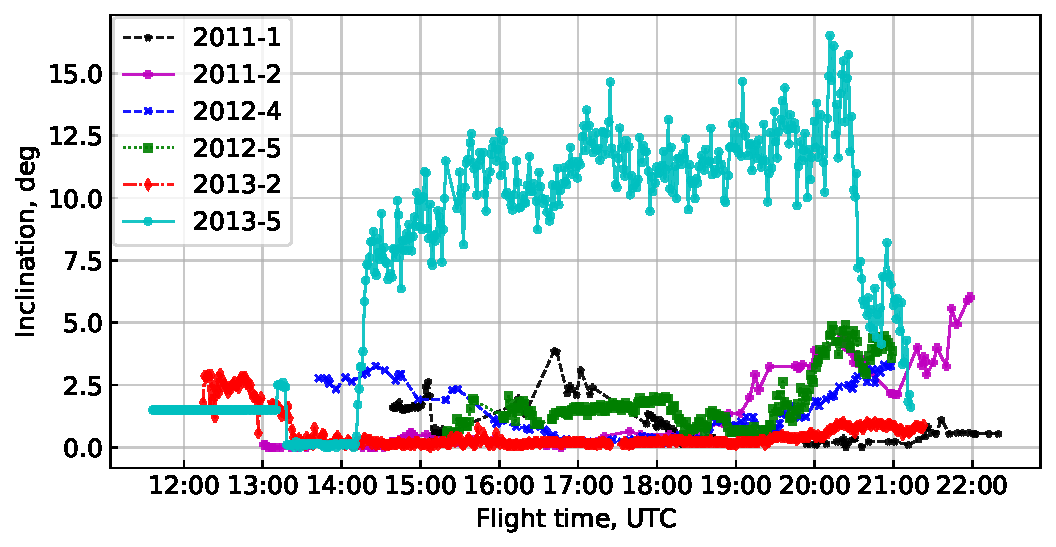
\includegraphics[width=\textwidth]{Telemetry_inclination.pdf}
       \caption{The detector inclination according to the inclinometer sensor during several flights in 2011-2013.}
    \label{fig:inclination} 
    \end{minipage}
    \hfill
    \begin{minipage}[t]{0.48\textwidth}
    \centering
       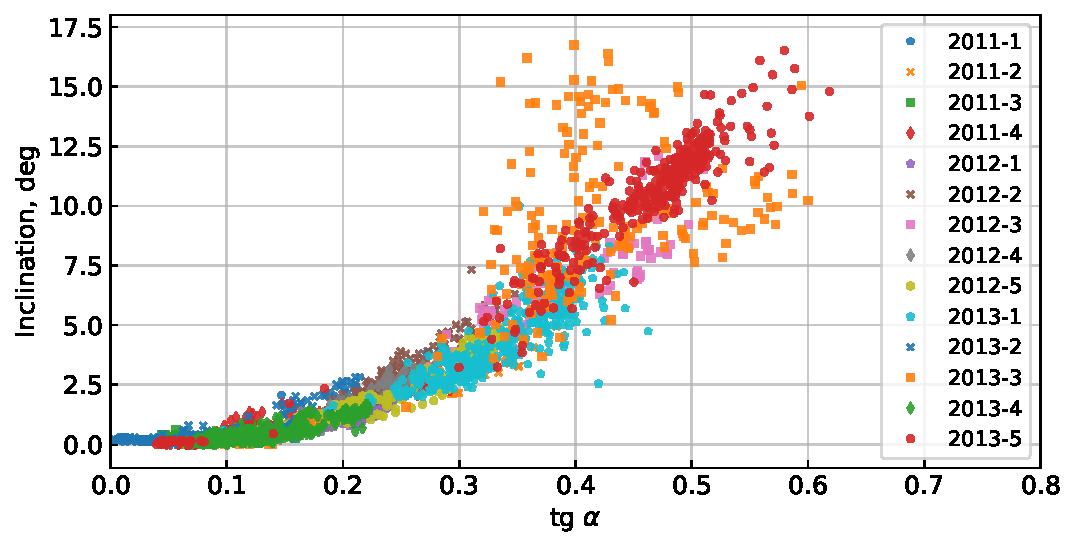
\includegraphics[width=\textwidth]{tg-inclination.pdf}
       \caption{Detector inclination against the detector drift from the start point to the detector altitude ratio which roughly translates into the tether inclination angle. See text for details on detector behavior.}
\label{fig:drift-inclination}
   
    \end{minipage}
\end{figure*}
%%%%%%%%%%%%%%%%%%%%%%%%%%%%%    

However, due to the construction of the SPHERE-2 detector suspension system to the balloon it was deflected to a certain degree by the wind in the direction away from the launchpad. In Fig.~\ref{fig:inclination} the inclination of the detector is shown for some flights in 2011-2013 runs. During some flights the detector was in a nearly vertical position (2011-1 of 2013-2), while in the others (2013-5) it was tilted to a significant angle. But this declination was steady and varied slowly over time. The maximum inclination angle recorded was about twenty degrees. In Fig.~\ref{fig:drift-inclination} the dependence of the detector inclination angle on the drift distance from the starting point relative to the flight altitude is shown for all experimental flights. The drift from the starting point divided by the flight altitude is as expected indicative of the wind strength which in turn defines the inclination angle. Strong fluctuations in flight 2013-3 (orange squares) occurred near midnight and coincided with rapid atmosphere profile change and weather worsening, the detector was landed prematurely. The detector inclination had a significant impact on the experiment `geometry' and was taken into account at the stage of EAS parameters reconstruction.

Detector altitude above lake surface according to the GPS data is shown in Fig.~\ref{fig:height}. The GPS module had some specific properties that resulted in some minor corrections into the altitude (detailed description see below in section~\ref{sect:gps_correction}). The surrounding air temperature and pressure  that were monitored for atmosphere propertied control are presented in the Fig.~\ref{fig:temperature} and Fig.~\ref{fig:pressure} respectively. Detailed description of the real atmosphere profile and overview of its impact on the data analysis is given below in section~\ref{sect:atmosphere-profile}.

%%%%%%%%%%%%%%%%%%%%%%%%%%%%%
\begin{figure*}[thb]    
    \begin{minipage}[t]{0.48\textwidth}
    \centering
 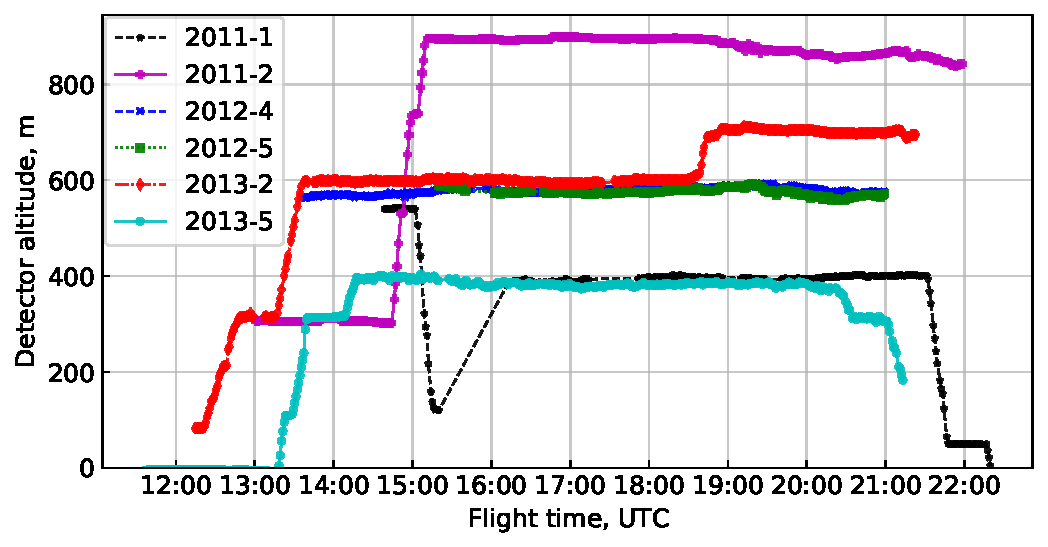
\includegraphics[width=\textwidth]{Telemetry_height.pdf}
    \caption{The altitude of the SPHERE-2 detector carried by the BAPA tethered balloon according to the GPS module data during 2011--2013.}
    \label{fig:height}
    
    \end{minipage}
    \hfill
    \begin{minipage}[t]{0.48\textwidth}
    \centering
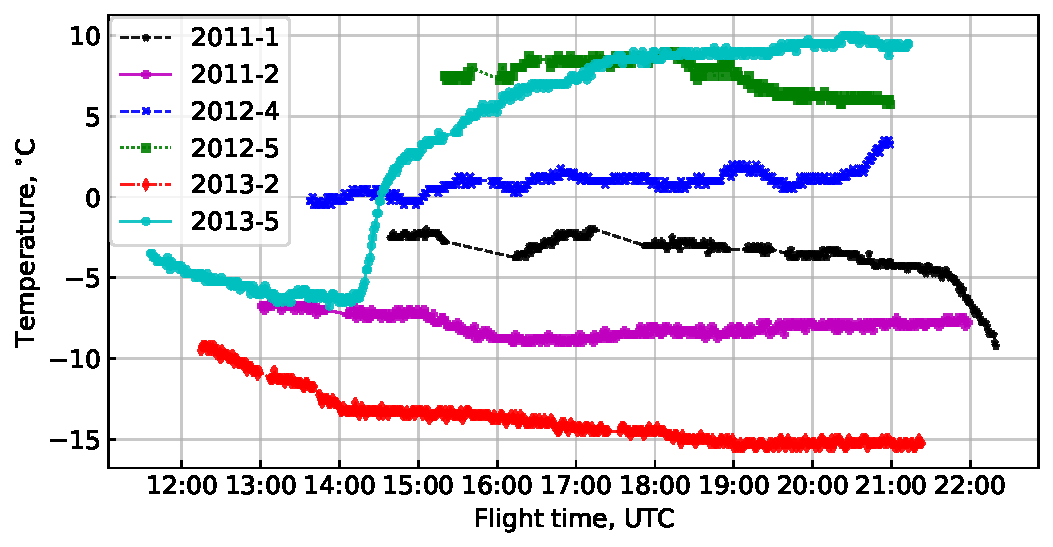
\includegraphics[width=\textwidth]{Telemetry_tmos.pdf}
    \caption{The air temperature near PMT mosaic during 2011--2013 runs.}
    \label{fig:temperature}
    
    \end{minipage}
\end{figure*}
%%  4 telemetry  pictures %%%
%%%%%%%%%%%%%%%%%%%%%%%%%%%%%

%%%%%%%%%%%%%%%%%%%%%%%%%%%%%
%% radius-inclination
\begin{figure}[tb]
    %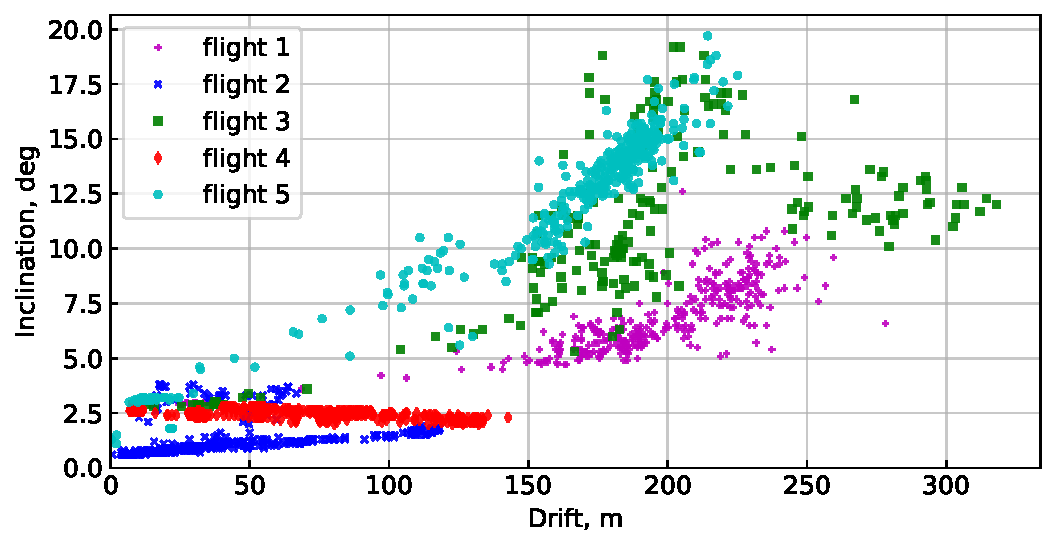
\includegraphics[width=0.48\textwidth]{radius-inclination.pdf}
    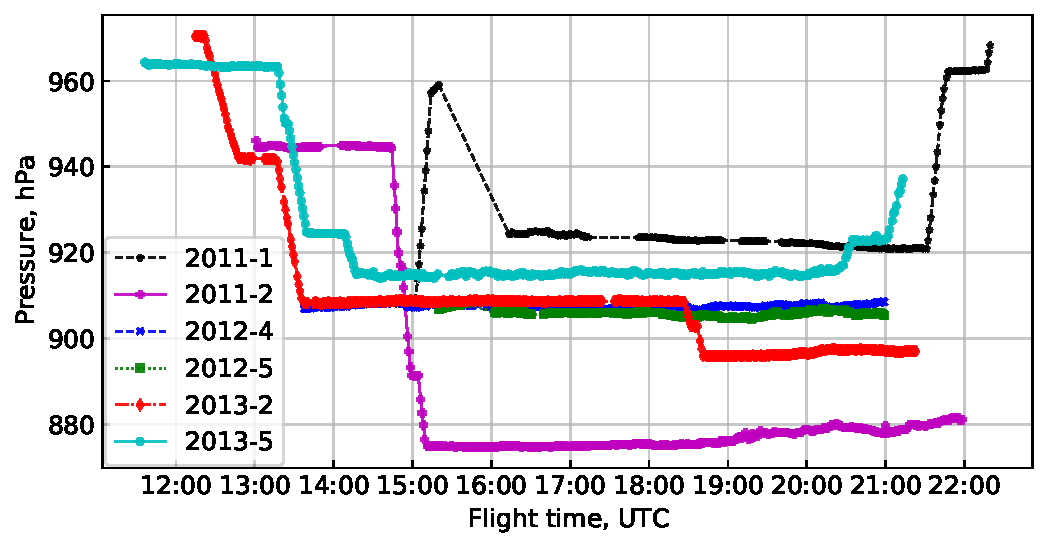
\includegraphics[width=.48\textwidth]{Telemetry_pressure.pdf}
    \caption{The air pressure according to the barometer sensor data  during 2011--2013 flights.}
    \label{fig:pressure}
\end{figure}
%%%%%%%%%%%%%%%%%%%%%%%%%%%%%


\subsection{PMT currents variations}

 The Fig.\ref{fig:current} shows the anode current of the detector mosaic central PMT for some of the flights. In 2008--2011 seasons on the central position was the FEU 84-3 PMT and in 2012--2013 seasons --- the Hamamatsu R3886 PMT. The latter has larger photocathode and amplification. Also for each flight the voltage on the PMTs was set independently and in some cases was changed mid-flight. The current increase in last minutes of 2011 flights was due to an increase in the illumination at the sunrise. In subsequent seasons the measurements were conducted at earlier dates so the sun rose later and did not affect measurements. But in general, the PMTs currents variations during the observations followed the variation of the background illumination of the snow.

%%%%%%%%%%%%%%%%%%%%%%%%%%%%%
%% The central PMT current %%
\begin{figure}[tb]
    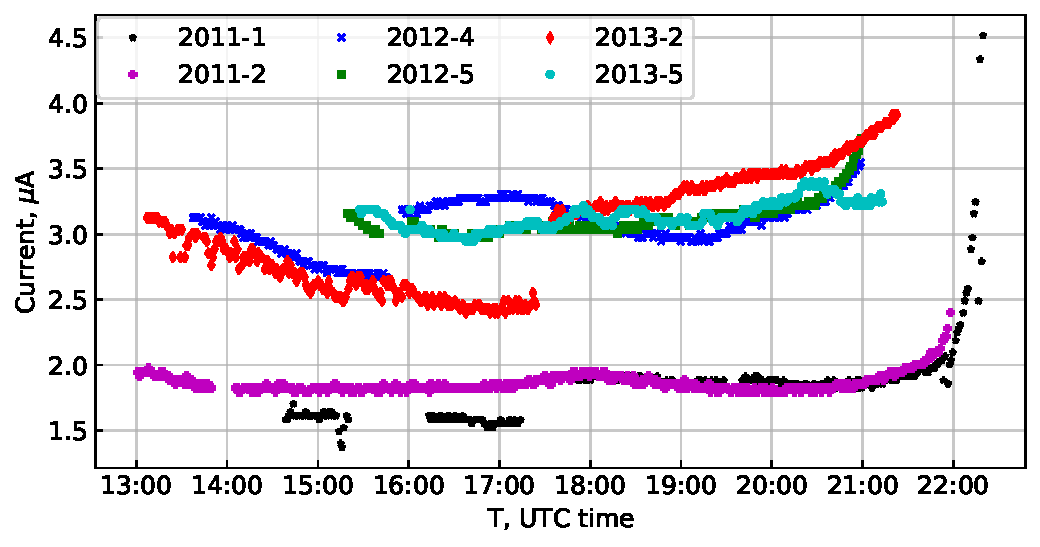
\includegraphics[width=0.48\textwidth]{hv-53.pdf}
    \caption{The central PMT currents in different flights.}
\label{fig:current}
\end{figure}
%%%%%%%%%%%%%%%%%%%%%%%%%%%%%

%%%%%%%%%%%%%%%%%%%%%%%%%%%%%%%%%%%%%%%%%%
%% 2012-3 currents
\begin{figure}[tb]
    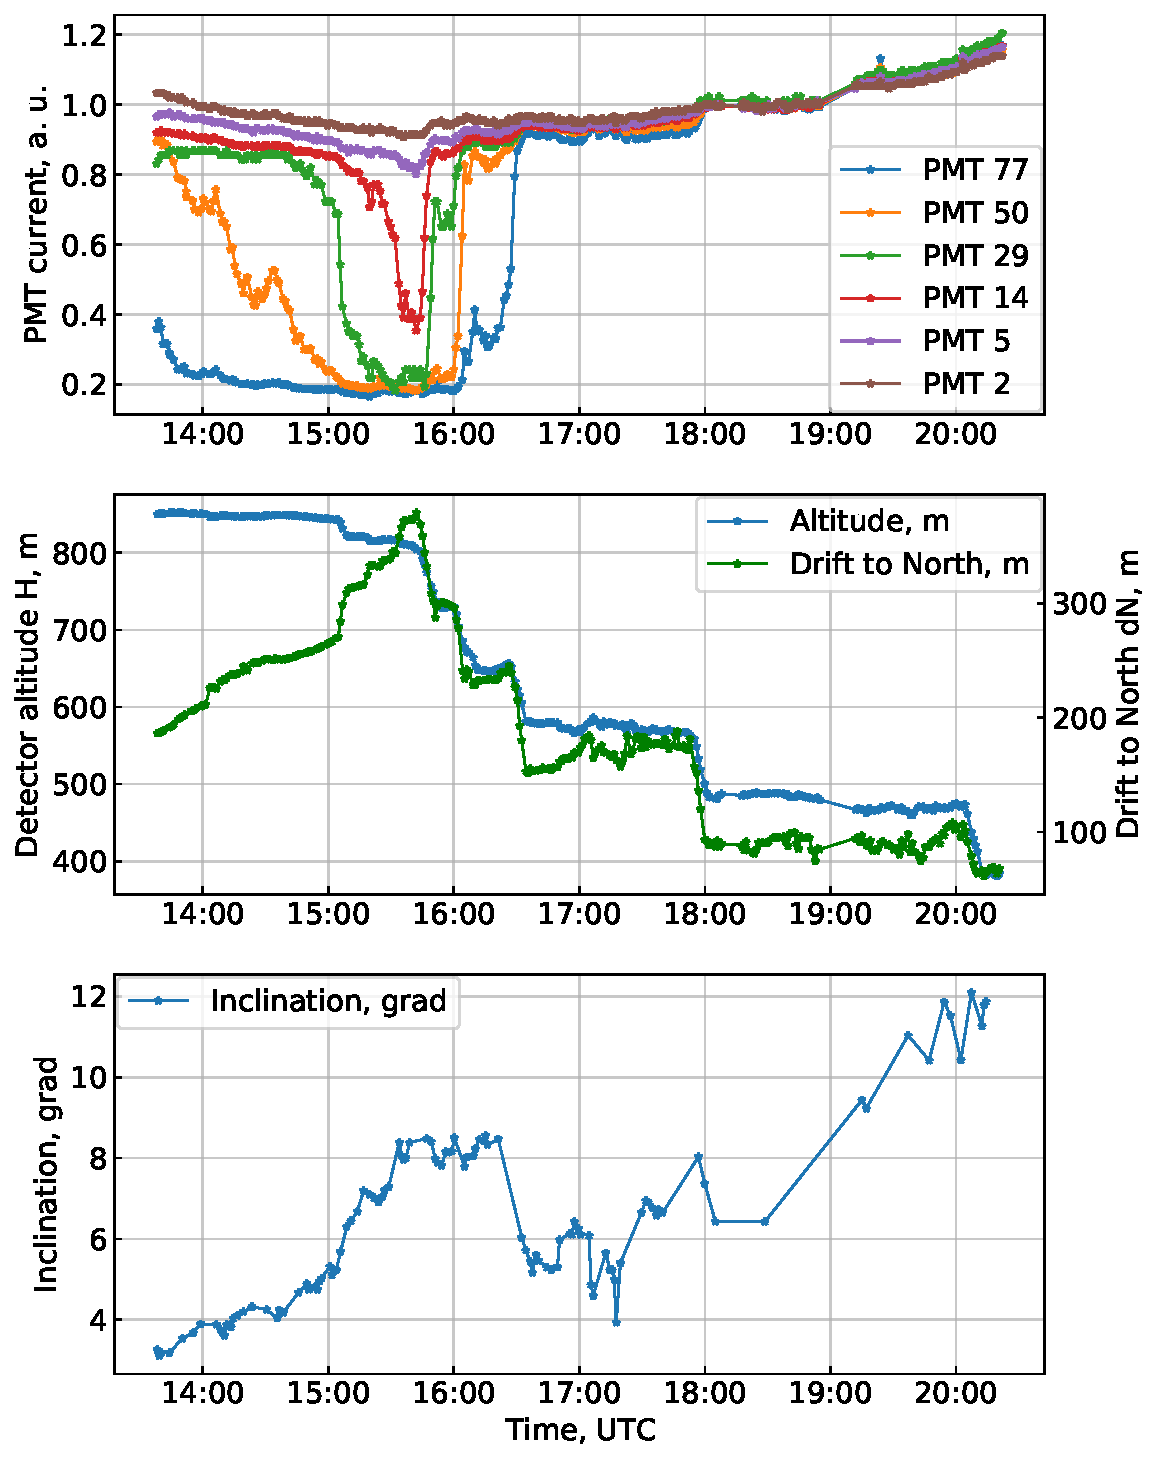
\includegraphics[width=0.48\textwidth]{2012-3_currents_H_dN.pdf}
    \caption{PMT currents, detector altitude, drift to the North, compass and inclination during flight 2012-3.}
    \label{fig:2012-3_currents}
\end{figure}

\begin{figure}[tb]
    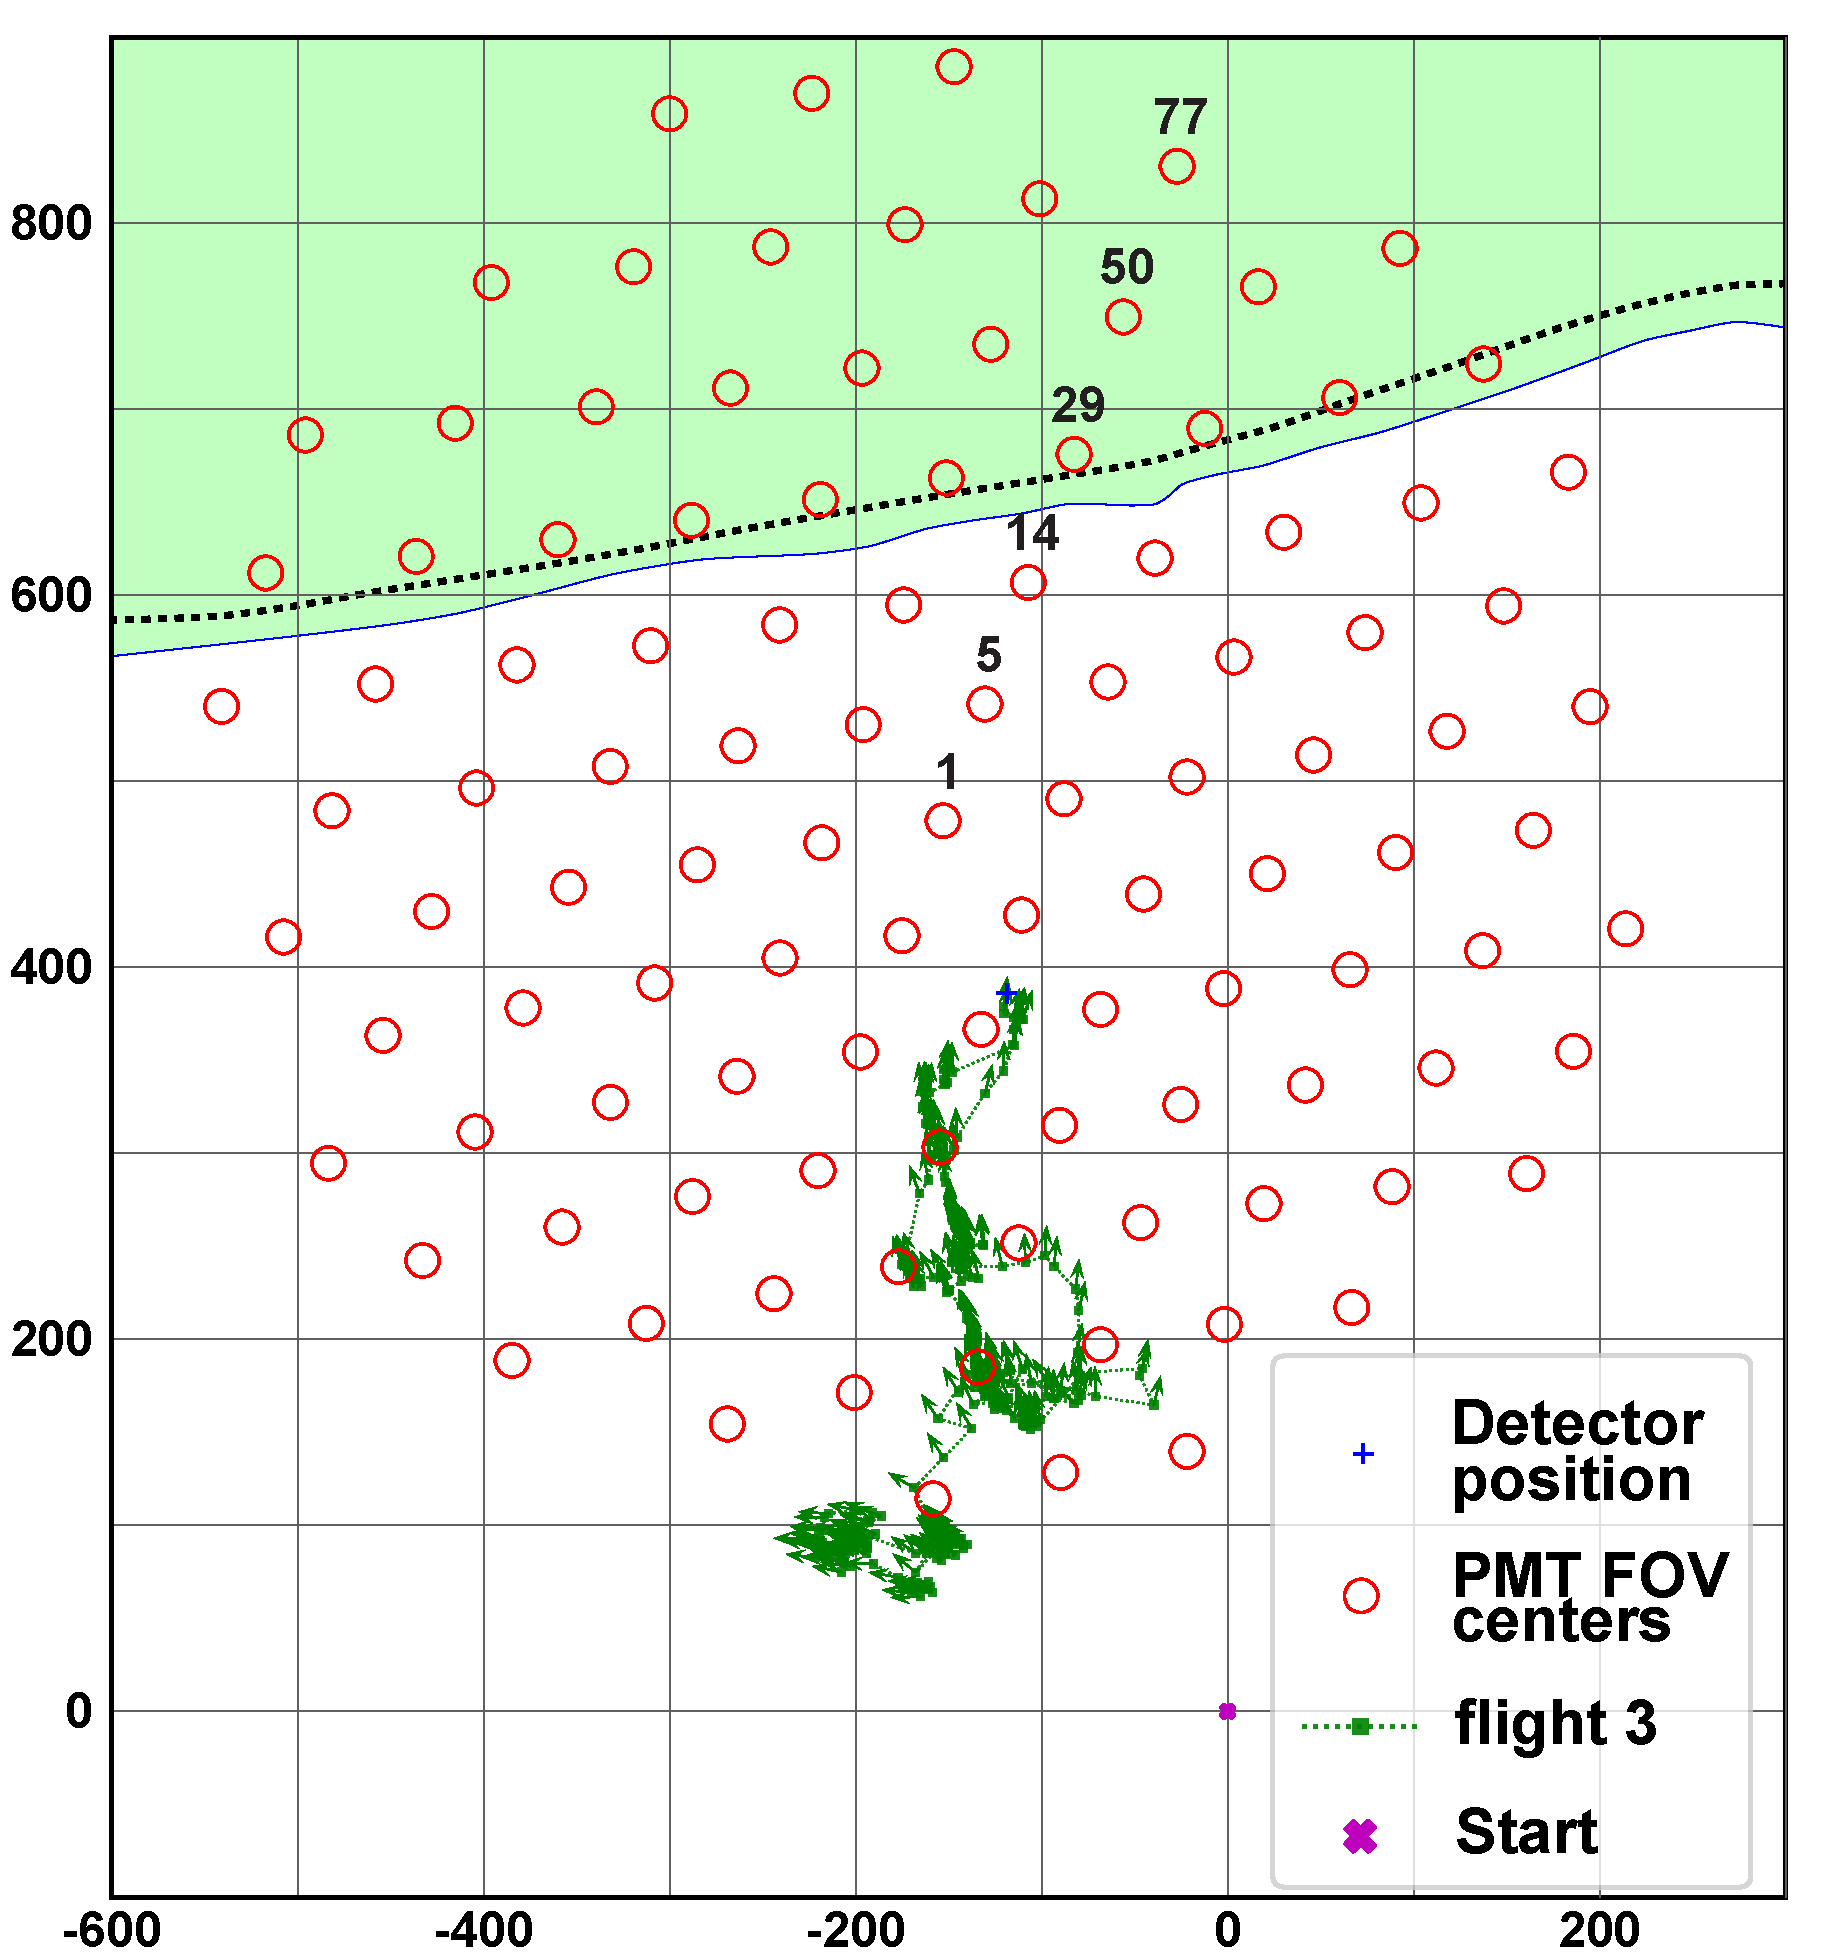
\includegraphics[width=0.48\textwidth]{2012_drift-mod.pdf}
    \caption{The SPHERE-2 detector drift in 2012-3 flight. Mosaic projection to the show surface is given for the time 15:47 UTC. Detector GPS position at that moment is indicated by the cross.}
    \label{fig:2012-drift}
\end{figure}

\begin{figure}[tb]
    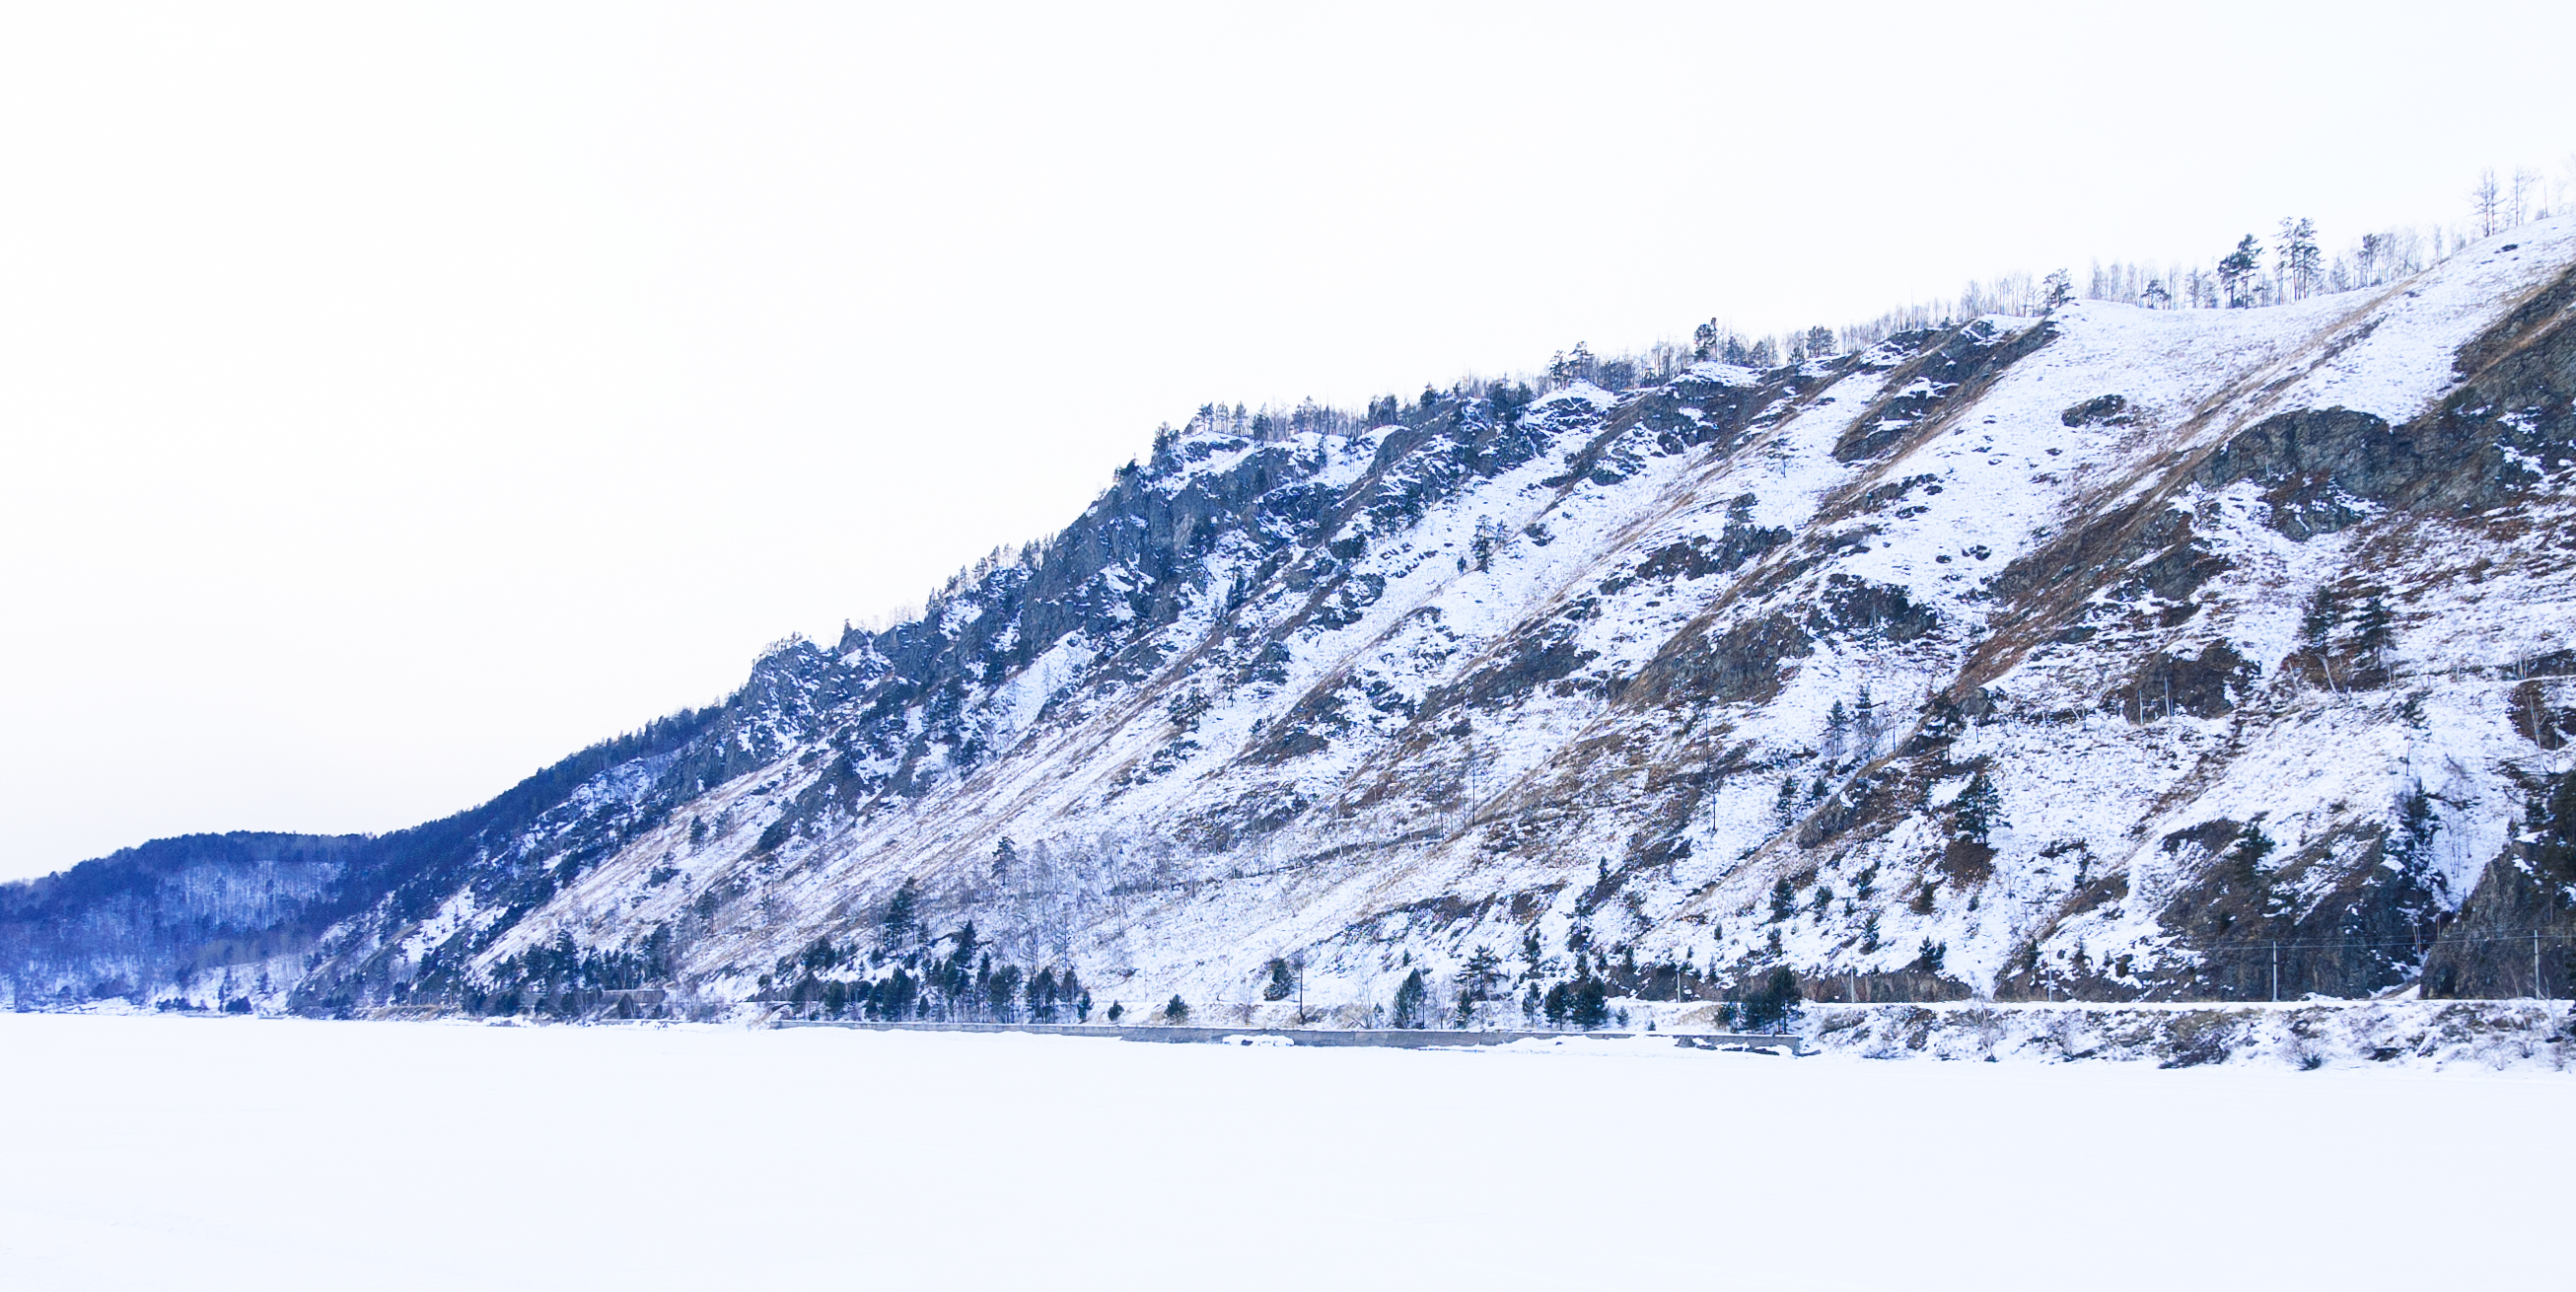
\includegraphics[width=0.48\textwidth]{DSC_7256_1.jpg}
    \caption{The view on the shoreline. The section `observed' by the detector from position indicated on Fig.~\ref{fig:2012-drift} is in the middle of the photo.}
    \label{fig:2012--shore-view}
\end{figure}
%%%%%%%%%%%%%%%%%%%%%%%%%%


However, in third flight of the 2012 season in part of the PMTs the abnormal drop of currents was observed (see Fig.~\ref{fig:2012-3_currents}).

%%%%%%%%%%%%%%%%%%%%%%%%%
\begin{figure}[tb]
\centering
    %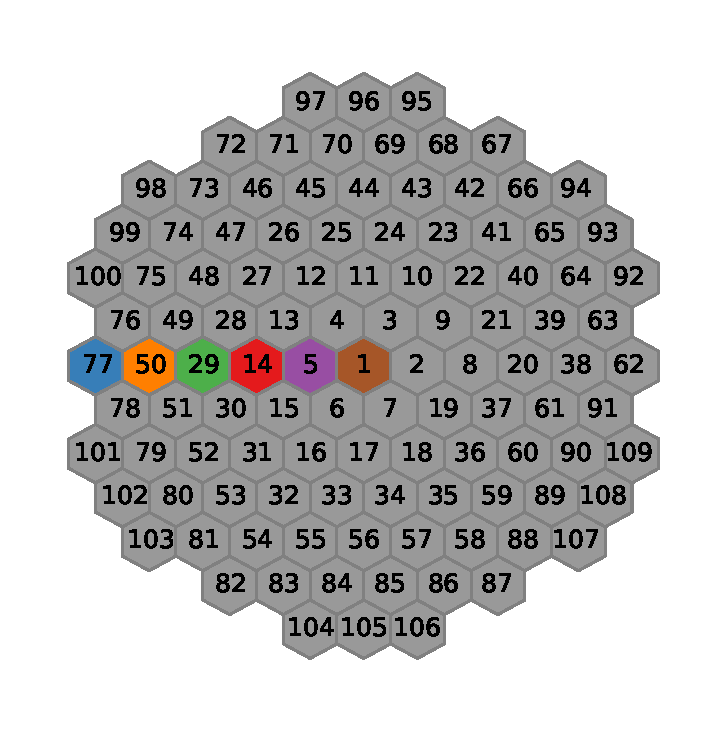
\includegraphics[width=0.2\textwidth]{2012-3_retina.pdf}
    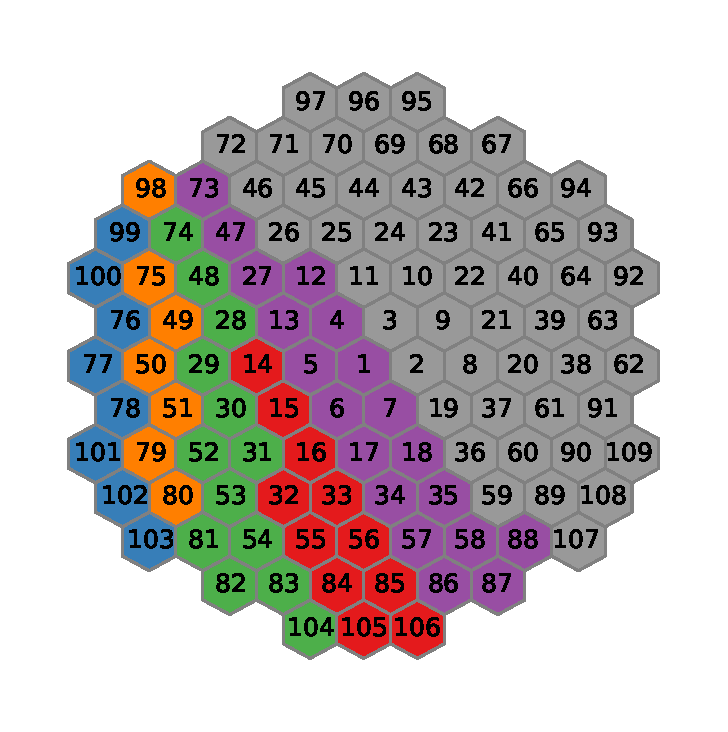
\includegraphics[width=0.35\textwidth]{2012-3_retina_all.pdf}
    \caption{The SPHERE-2 PMT mosaic scheme. PMT numbers are indicated. PMTs are colored according to it current curve type in 2012-3 flight with colors as in Fig.~\ref{fig:2012-3_currents}.}
    %\todoi{Выберите одну из двух.}
    \label{fig:2012-3_shore_image}
\end{figure}
%%%%%%%%%%%%%%%%%%%%%%%%%%%%%

The registered currents in some PMTs (numbers 5, 14, 29, 50 and 77) are shown in Fig.~\ref{fig:2012-3_currents}~(top panel). These PMTs form a straight line on the PMT mosaic and the currents dropped and restored in them in the same order they are positioned in the mosaic. There were more PMTs with current drop occurring at the same time. In Fig.~\ref{fig:2012-3_shore_image} the PMTs are colored according to similar current drop and restore times.

This anomaly was observed in the the first half of the flight during the observations at 850~m altitude. At that time according to GPS the balloon was drifting north from starting point. Detector altitude and drift are shown in~Fig.~\ref{fig:2012-3_currents}~(central panel). Due to the wind becoming stronger on that altitude the balloon was subsequently lowered to the 480~m altitude and the currents had returned to their normal behaviour. 

The analysis of the detector position and tilt showed that it at that time was observing the part of the shoreline and behind. At this location the shoreline is a narrow artificial ledge built for the railroad and further changes into a steep snow-less cliff wall with trees atop (see Fig.~\ref{fig:2012--shore-view}). The reflective properties of both rock and pine trees is way lower than that of a snow. In Fig.~\ref{fig:2012-drift} the detector trajectory (green line), starting point (purple cross) are given. The detector position (blue cross) and corresponding PMTs centers projections (red circles, the exact shapes of each PMT field of view are discussed below in) on to the snow are given for 15:47 UTC, the moment of the highest currents drop and furthest north drift. The currents behavior in each PMT is consistent with its crossing the shoreline. The PMTs that show no currents drop by our estimations always observe the clear snow surface. In all other flights no instances of detector drift to the shore was observed.

This in itself confirms the consistency of the detector orientation and position monitoring.

\section{Telemetry analysis}
%%% Переименовать и пересортировать

The position and inclination of the SPHERE-2 detector are the important values to correct reconstruction of the registered EAS Cherenkov light characteristics. In contrast to Cherenkov ground-based arrays, such as~\ref{}\todoi{ссылки на Якутск и Тунку}, the SPHERE-2 detector has a variable recording area depending on both the altitude and the inclination.

%%%%%%%%%%%%%%%%%%%%%%%%%%%%%%%%%%%%%%%%%%%%%%%%%%%
\subsection{GPS altitude correction with barometer data}
\label{sect:gps_correction}

Thorough telemetry data analysis revealed that at some periods of time recorded GPS data for altitude was inadequate. Namely, after rapid changes in altitude due to the balloon ascent or descent the GPS height lagged behind corresponding pressure change and varied in a smoothed fashion. The example of such behavior is shown in Fig.~\ref{fig:h_corr}, top panel. We were unable to find out the exact source of this distortion, but our best guess is that it's a result of GPS module's internal error correction algorithm. Module's primary application is naval/aerial navigation~\cite{GPS-module-specs} and it may interpret sudden change in altitude without proper horizontal speed as an error.

\begin{figure}[tb]
    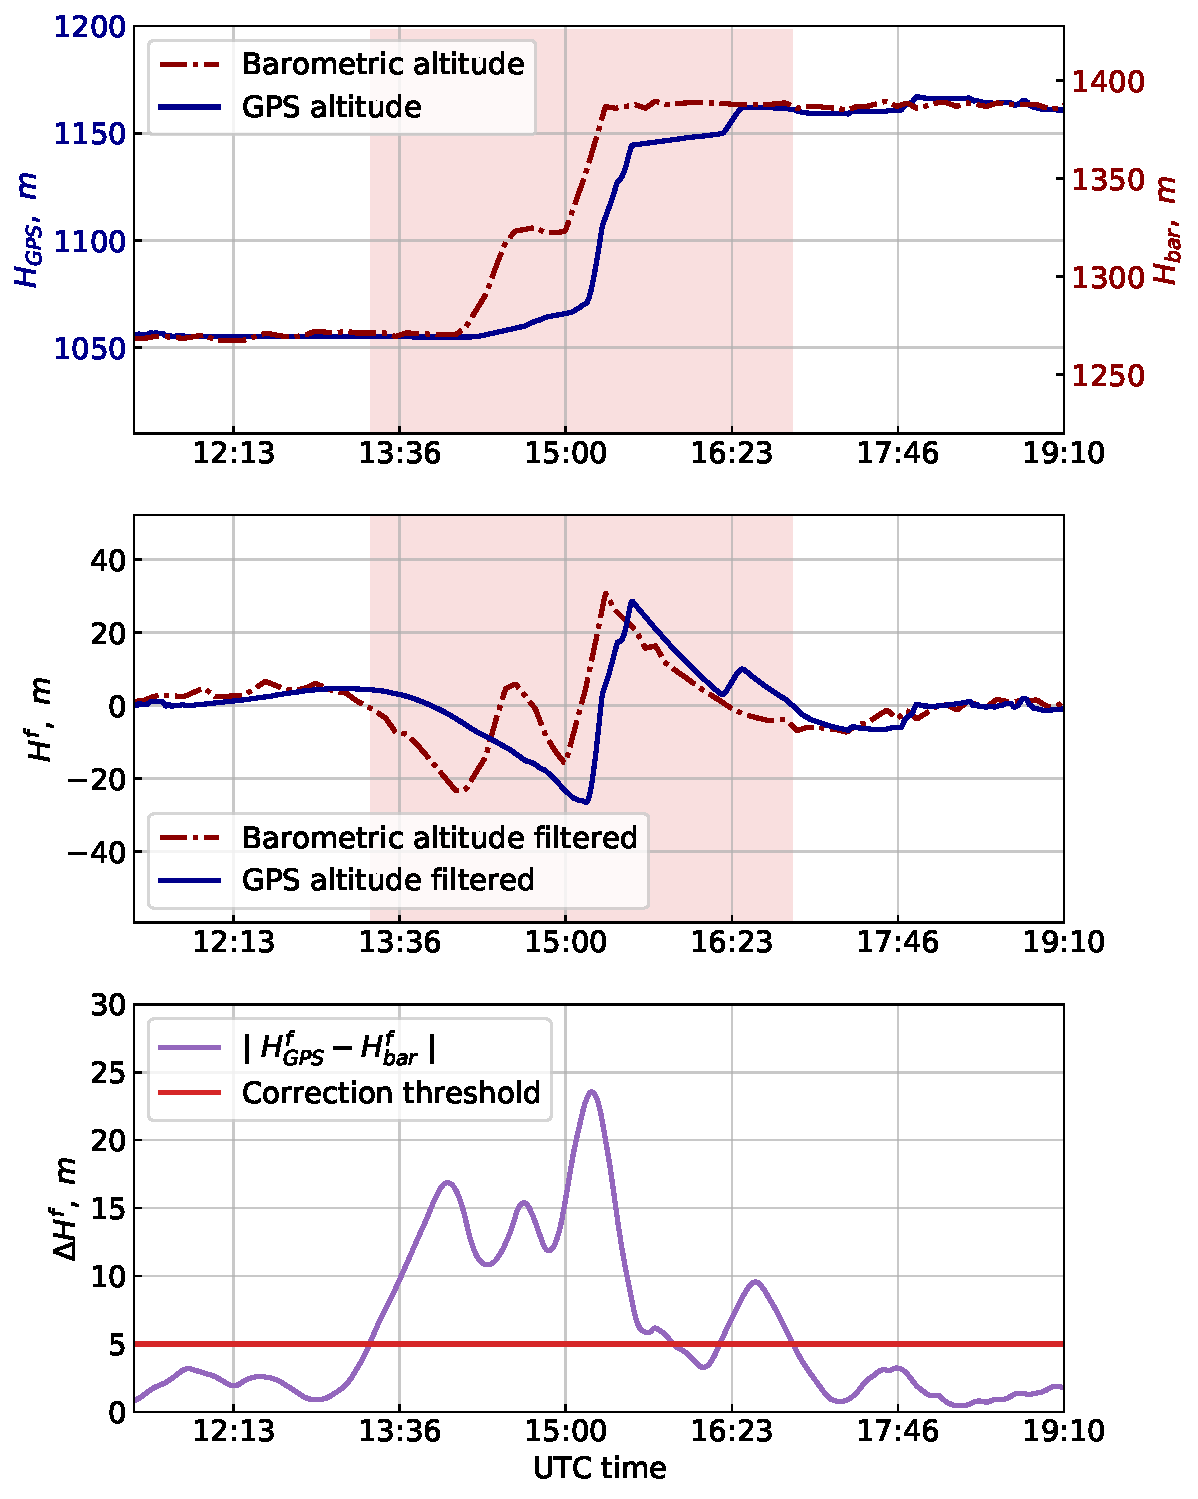
\includegraphics[width=0.48\textwidth]{height_correction.pdf} 
    \caption{Example of anomalous GPS altitude behavior, compared with `barometric' altitude (top panel) during flight 2013-2. Same data with high-pass digital Butterworth filter applied (middle panel). Smoothed absolute delta of high-passed altitudes from middle panel, used as gate with threshold set at red line; intervals above this line correspond to red bands on other panels, which are the intervals subjected to GPS data correction.}
\label{fig:h_corr}
\end{figure}

\begin{figure}[t]
    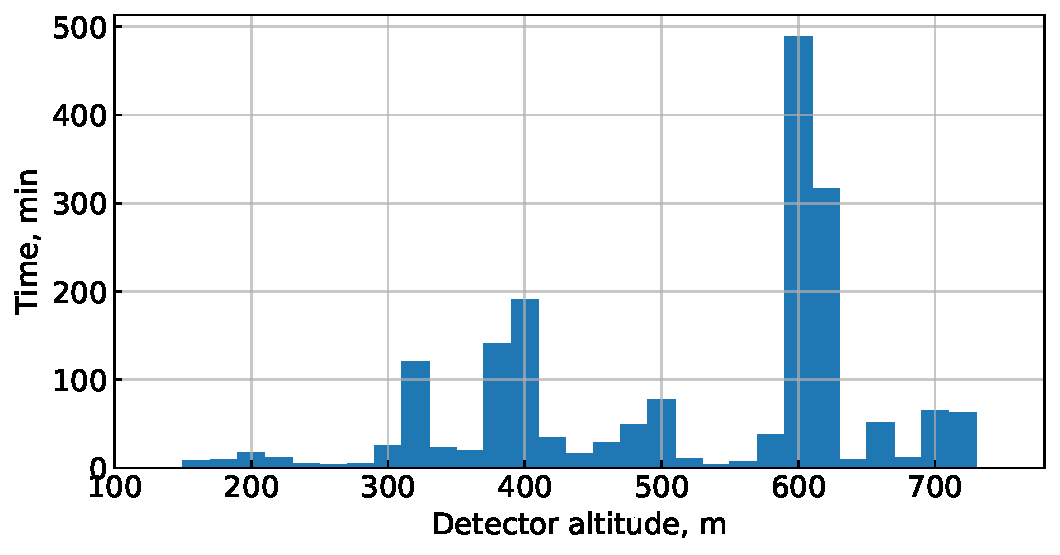
\includegraphics[width=19pc]{time_on_altitude.pdf}%
    \caption{The altitude distribution of experiment time.}
    \label{fig:time_on_altitude}
    \todoi{Обновить картинку по исправленным высотам.}
\end{figure}

Affected time intervals are relatively short for most flights, but during them some events were recorded\todoi{Сколько событий, надо указать точно.}. In order to correctly estimate detector altitude for those events, and to maintain overall data consistency we attempted to correct these smoothed GPS altitude measurements using pressure data from barometer, which has strong and well-understood dependence on altitude.

First of all, to identify affected time intervals we calculated approximate `barometric height' from pressure data using inverted barometric formula $H_{bar} = H_0 - a \log (P/P_0)$ with parameters $H_0 = 456~\textrm{m}$ (Baikal surface level), $P_0 = 1000~\textrm{hPa}$ (close to average March pressure on the Baikal surface) and $a = {RT}/{Mg} \approx 8400~\textrm{m}$ (standard value for barometric formula). Next, we had applied a high-pass digital Butterworth filter to both GPS and barometric altitude data to compare only fast variations of both values. Cutoff frequency for filter was set to $0.416~\textrm{mHz}$ ($T=40$ min with telemetry data being recorded each $10~\textrm{sec}$) and slope was set to around $12~\textrm{db per octave}$. Resulting high frequency components are shown on Fig. \ref{fig:h_corr}, middle panel.

It is clear that for stable altitude and valid GPS measurements GPS and barometric height are subjected to fast, somewhat correlated fluctuations (they are not completely correlated probably due to GPS error of the order a meter). In contrast, intervals of smoothed GPS data show divergence of these two values. We calculated delta between filtered GPS and barometric altitudes and applied moving average with $6~\textrm{min}$ window. We then identified intervals for correction as those that feature the smoothed delta above a threshold of $5~\textrm{m}$ in absolute value. The threshold was chosen so that in regular conditions the smoothed delta did not exceed it, as it has normal-like distribution with standard deviation of around $3~\textrm{m}$. Smoothed delta with the threshold are shown in Fig.~\ref{fig:h_corr}, bottom panel; correction interval is shown on top panel with red band.

After intervals were picked, for each of them we found two adjacent intervals $2~\textrm{min}$ each with correct GPS data and once again used barometric formula to estimate actual altitude inside the interval. In this case it is used to describe local behavior of $H(P)$. We fitted $(P, H)$ data points from adjacent regions with the same barometric function and replace smoothed GPS data with the new `local barometric height'.

The total duration of the intervals subject to corrections was small. The total distribution of the time spend by the detector at each height is presented in Fig.~\ref{fig:time_on_altitude}. Most of the time the detector spent at 400, 500, 580 and 890~m, However, the actual distribution of registered events across the altitude is a more complex question since the trigger settings and overall detector performance changed over time and across seasons. Careful analysis of this question will be covered in following publications.

\subsection{Atmosphere density profile}
\label{sect:atmosphere-profile}
%%% Atmosphere profiles figures %%%%
\begin{figure}[bt]
\centering
\begin{minipage}[t]{0.48\textwidth}
    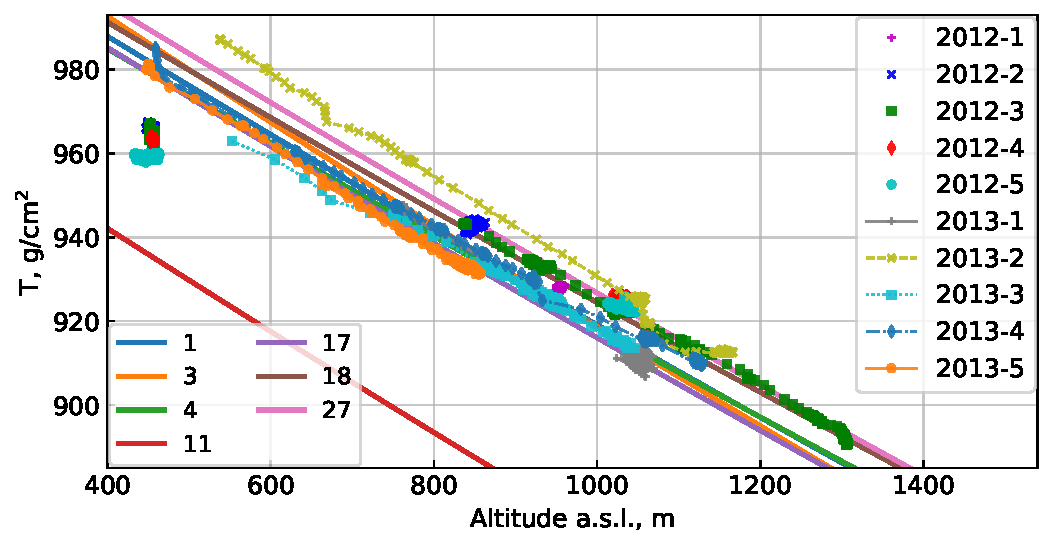
\includegraphics[width=\textwidth]{figs/atmosphere_T.pdf}
    \vspace{-1.0pc}
    \caption{Mass overburden versus altitude experimental data (points) in each flight and CORSIKA profiles (solid lines with corresponding models numbers). For preliminary SPHERE-2 modeling and analysis the N0 11 atmosphere was used.}
\label{fig:massoverburden}
\end{minipage}
\vfill
\vspace{1pc}
\begin{minipage}[t]{0.48\textwidth}
    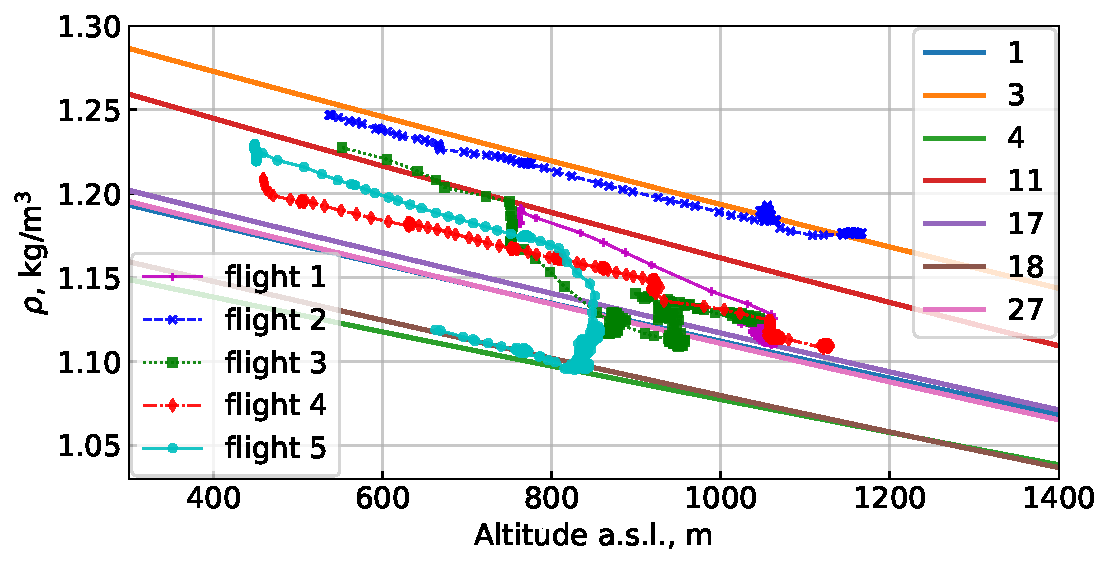
\includegraphics[width=\textwidth]{figs/atmosphere_rho.pdf}
    \vspace{-1.0pc}
    \caption{Density versus altitude experimental data (points) in each flight and CORSIKA models density profiles (solid lines) same as in Fig. \ref{fig:massoverburden}).}
\label{fig:density}
\end{minipage}
\end{figure}

%%%%%%%%%%%%%%%%%%%%%%%%%%%%%%%%%

After the corrections to GPS altitudes were applied the atmosphere density profiles were reconstructed. Direct measurements with on-board barometer and thermometer were taken at less than 1000~m above the ice therefore information about higher atmosphere is not available. To obtain the best extrapolation of these data we had to use the set of previously measured and parameterized atmospheres provided in CORSIKA software~\cite{hec98}.

In CORSIKA the atmosphere is described in terms of mass overburden $t(H)$ that is parameterized as a piecewise continuous function which has exponential behavior in the lower four layers and linear in the highest one. %Since the $T(H)\equiv \int_{h}^{+\infty} \rho(x) dx$.
%Layer boundaries are selected in a manner that the overall function $T(h)$ can be differentiated continuously. 
CORSIKA provides 26 atmosphere models corresponding to measurements taken at different seasons in different locations around the globe. For each atmosphere experimental range of altitudes was fully contained in the lowest layer.

We used following equations to derive mass overburden $t$ and density $\rho$ from measured pressure $p$ and temperature $T$.

\begin{equation}
t     = \frac{p}{g}, \\
\rho  = \frac{p \, M}{R \, T} \\
\end{equation}

Here $g$ is the gravitational acceleration, $M$ is the average molar mass of air, $R$ is the gas constant.

Calculated experimental points for $t$ and $\rho$ in each flight are shown in Fig.~\ref{fig:massoverburden} and Fig.~\ref{fig:density} respectively. CORSIKA atmospheres are shown with solid lines,The profile that was adopted in the preliminary modeling (atmosphere model No 11) is shown with red line.

From this comparison follows that previously picked atmosphere is inconsistent with experimental data for $t$ in terms of absolute values, but their derivatives lie relatively close. Therefore either full remodeling with better fitting atmosphere or some correction of final data is required to reduce systematic errors in energy and composition estimations.

%% влияние атмосферы на высоты генерации света на (Галкин)
%%% === Table CORSIKA
\begin{table}[t]
\centering
\caption{Cherenkov number ratios for different CORSIKA atmosphere model pairs: means, variations, relative variations. 10 PeV primary protons. Zenith angle 15 $\deg$. Sample volume 30 events.}
\label{tab:atmmod}
\vspace{1pc}
\begin{tabular}{|c||c|c|c|}
\hline
model pair  & mean &  variation   & relative variation \\ 
            &  $m$ & $\sigma$     & $\sigma/m$          \\ 
\hline 
\hline 
 3/4 &  1.015    &  0.0490     &   0.0483   \\
\hline
11/3 &  0.9834    &  0.0511     &   0.0520    \\
\hline
11/4 &  0.9963    &  0.0443     &   0.0445    \\
\hline
\end{tabular}
\end{table}


%%% === LDF Calculation
\begin{figure*}[tb]
 \begin{minipage}[t]{0.48\textwidth}
    \centering
    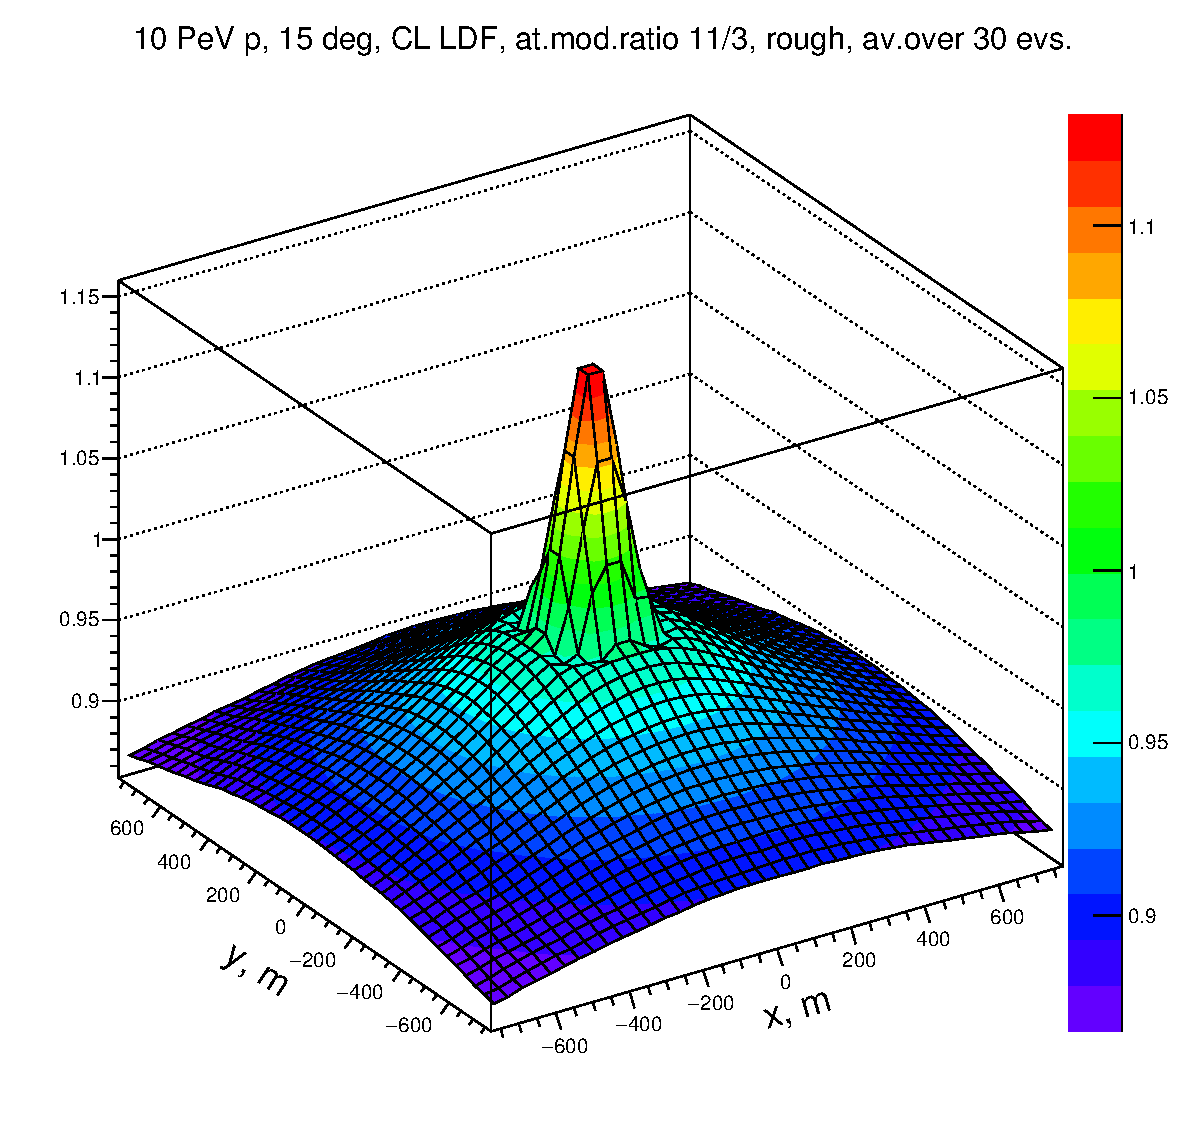
\includegraphics[width=19pc]{11d3}%
    \vspace{-1.0pc}
    \caption{Sample mean Cherenkov light lateral distribution ratio for CORSIKA atmosphere model
    pair 11/3. Bin size 50~m $\times$ 50~m. 10~PeV primary protons. Zenith angle 15~$\deg$. Sample volume 30~events.}
\label{fig:3d11}
\end{minipage}
\hfill
\begin{minipage}[t]{0.48\textwidth}
    \centering
    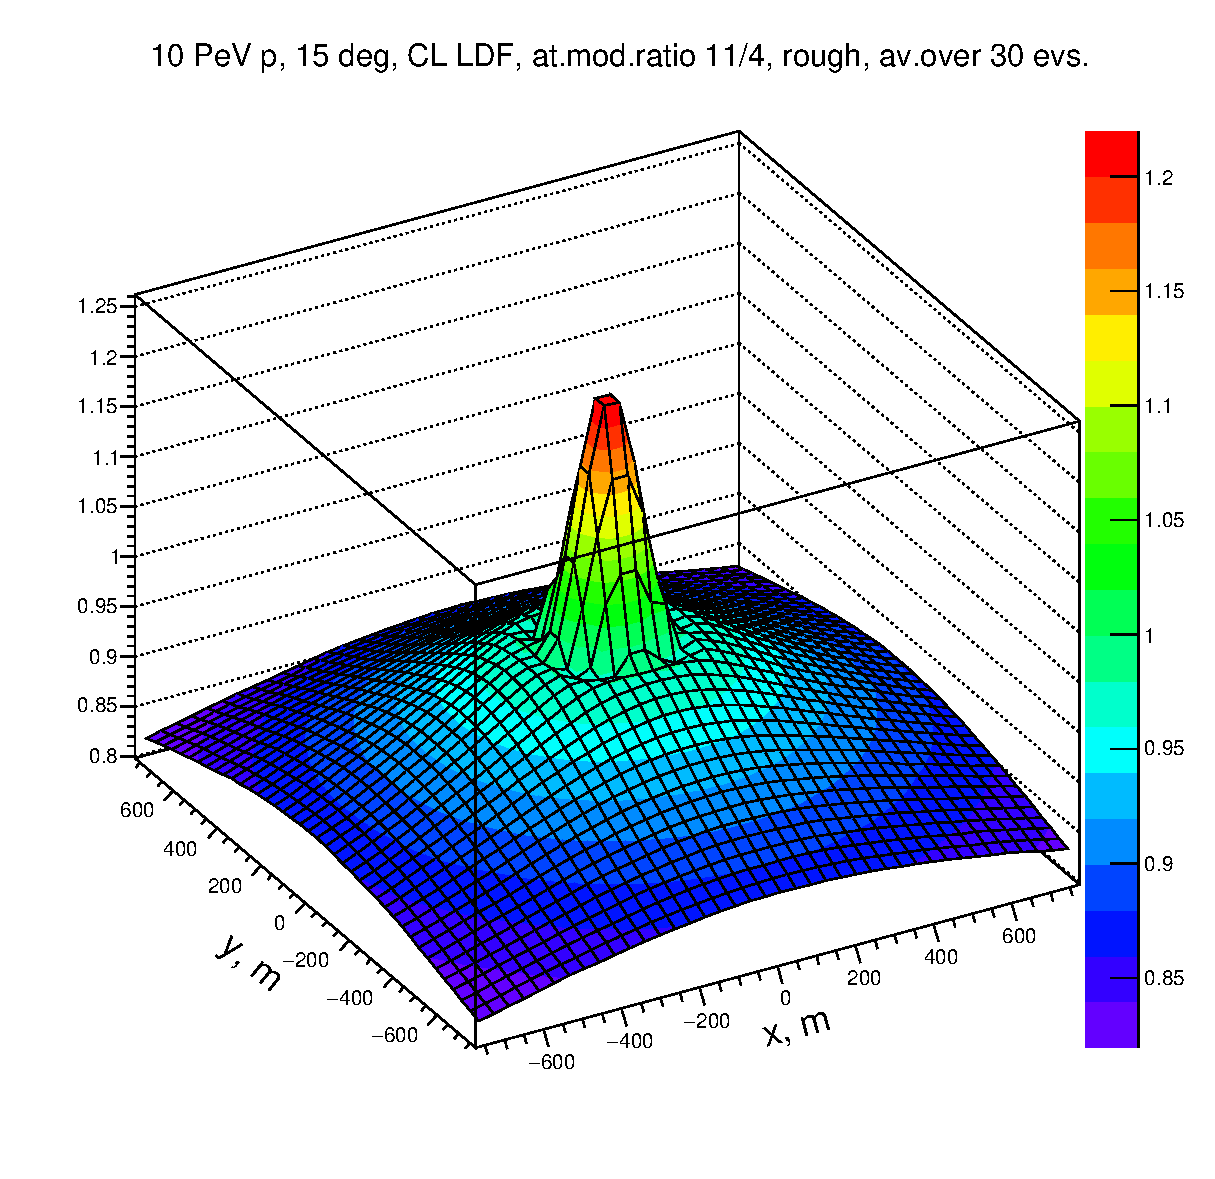
\includegraphics[width=19pc]{11d4}%
    \vspace{-1.0pc}
    \caption{Sample mean Cherenkov light lateral distribution ratio for CORSIKA atmosphere model
    pair 11/4. Bin size 50~m $\times$ 50~m. 10~PeV primary protons. Zenith angle 15~$\deg$. Sample volume 30~events.}
\label{fig:4d11}
\end{minipage}
\end{figure*}


CORSIKA atmosphere model 11 was used all through the modeling runs. Modeling lasted for about 2 years and at that time it was not possible to choose an atmospheric model close to reality. The use of the experimental points in $t$ or $\rho$ cannot provide a reasonable  choice of the model, it can only give us some clue as to what the model should be. Full-fledged choice must include data on vertical profile of atmosphere layer up to altitudes at least 20 km above the lake Baikal level because the Cherenkov light mostly comes from this layer. Still we can make some conclusions on the atmosphere model effect on primary energy and mass estimates by comparing the artificial showers simulated for different models.

We produced such artificial events initiated by 10~PeV protons for a number of models, passing close to the experimental $t$ and $\rho$ trajectories, and CORSIKA model 11. The results are expressed as ratios of full numbers of Cherenkov photons and lateral distribution functions.

The lateral distributions were calculated within a vast (3.2km $\times$ 3.2km) carpet tiled with 2.5~m $\times$ 2.5~m squares but for the purpose of the comparison were smoothed by integrating over 50m $\times$ 50~m squares approximately imitating the sensitivity spots of telescope pixels.

Sample volume for each model was 30 showers. Table~\ref{tab:atmmod} shows mean values and variations of Cherenkov photon number ratios for three pairs of CORSIKA atmosphere models (3/4, 3/11 and 4/11). The ratios of sample mean lateral distributions for 3/11 and 4/11 pairs are shown in Fig.~\ref{fig:3d11} and Fig.~\ref{fig:4d11}, respectively. Pair 3/4 reflects maximum effect of atmosphere model choice from the viewpoint of experimental $t$ and $\rho$ measurements. Pairs 3/11 and 4/11 compare the model 11 used in simulations to the models approximating the experimental data.

Table data clearly states that substantial changes of atmosphere model affect the total number of Cherenkov photons and thus the primary energy estimates not more than by 5\% on average. Conclusions on primary mass estimates are not so clear but the lateral distribution ratio plots indicate some changes in CL LDF of about 6 to 12\% (12 to 20\%) near the shower core, closer than 80 m, and about -2 to +6\% (0 to +12\%) in 80--150m circle for 3/11 (4/11) pair, which definitely might affect our mass-sensitive criterion. More accurate evaluation of the effect will be given elsewhere.


%%%% === mosaic picture ===
%\begin{figure}[tb]
%\centering
%    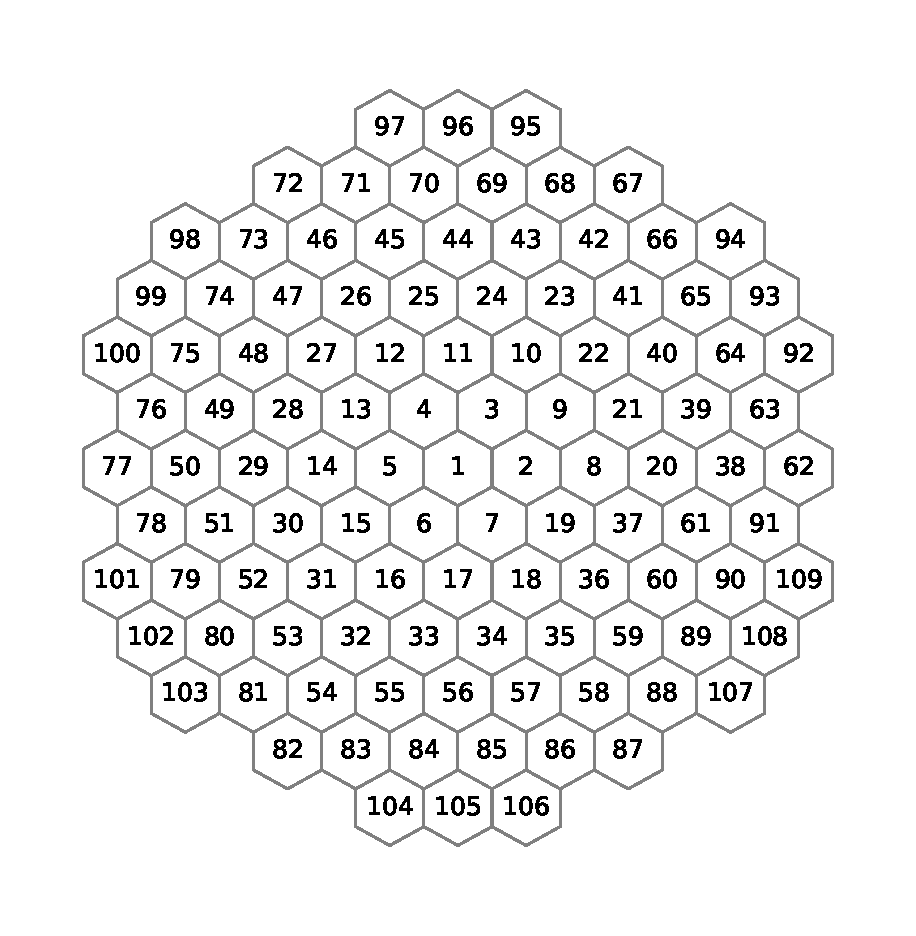
\includegraphics[width=19pc]{mosaic.pdf}%
%    \vspace{-1.0pc}
%    \caption{The PMT mosaic of the SPHERE-2 detector with PMTs numbers indicated.\todoi{Грохнуть!}}
%\label{fig:mosaic}
%%\end{minipage}
%\end{figure}


%\subsection{PMTs' field-of-views correction}
%\label{sec:PMTFOV}

%In flight during measurements whenever the detector become inclined, the configuration of it's field-of-view (FOV) changed. The FOV of some PMTs shrunk and got closer to the central PMT FOV, for others got larger and moved further from the central PMT FOV. This change of PMT FOVs distorted the reconstructed Cherenkov LDF in spatial terms. Also, change in FOV orientation meant change in optical distance from which the PMT collects light (which affected time measurements). Another issue was the relevant change in average angle under which the snow surface was observed by PMT, which changed light scattering effectiveness (and this distorted the LDF in terms of signals values). In other words, the mosaic inclination if compared to the ground based experiments resulted in measuring stations repositioning with grid distortion and in gradual change in stations sensitivity.

%In addition to the full Monte Carlo simulation of the SPHERE detector described in~\cite{Ant19} the calculations of detector's optics and PMTs' FOV was performed. The detectors optical scheme is presented on the Fig.~\ref{fig:optics}. 

%\todoi{Сократить}
%%%%The detector was set at 1000~m altitude with zero inclination above flat horizontal observation level. The ground level was divided by the square mesh $[X;Y]$ with 1~m step. From each ground square the weighted photons were emitted towards the detectors diaphragm. The diaphragm was divided into $[x;y]$ mesh with 5~mm step. From each ground square a total of 25600 photons were emitted towards the detector. Each photon weighted by the snow reflection coefficient $k_{snow}$ (taken as 0.95~\cite{war82}), by the $\cos^2(\theta)/2$ to account for Lambert scattering (the $\theta$ is the angle between the direction to the detector and Z-axis), by the distance factor $2\pi{}S/(H^2+(X-x)^2+(Y-y)^2)$ and additional $\cos\theta$ to account the non-normal ray incidence on the diaphragm and the the normalization coefficient of 2.

%%%%At the detector diaphragm level the photons were checked whether they passed the the diaphragm successfully or not and were traced further. At the mosaic level (the mosaic geometrically is a domed truncated cone) the photons were checked that they missed back side of the mosaic and were traced further to the mirror. At the mirror the photons were reflected and additionally weighted by the mirror reflection coefficient $k_{mirr}$. During different seasons of observations this coefficient changed as the mirror degraded, so for data analysis the coefficients were selected accordingly to {\color{red} measured ones}, $k_{mirr}$ was about 0.75--0.80 during 2011--2012 seasons and $k_{mirr}$=0.95 for the new mirrors in 2013. After the photons were reflected by the mirror, they were traced back to the mosaic level and check for successfully hitting it. At this step the photons were checked whether they hit any PMT or mosaics blind material. The \mbox{FEU-84-3} PMT's photocathode has 26~mm diameter sensitive area. The spacing between photocathode centers in out mosaic was 44.5~mm, so only 30\% of the mosaic was sensitive to the light. For each photon at the PMT glass surface the glass mirroring coefficient $k_{PMT}$ was calculated, the photon's polarization was selected randomly.

%For fixed altitude (1000~m) and vertical detector orientation a full ray-tracing simulation was performed using dense grid ($1\times1$~m square) across the snow surface with weighted rays that accounted for distance to the mosaic, snow reflective properties, mirror efficiency and reflections on the PMT outer surface. Tracing photons from the full ground grid allowed to find each PMT's FOV and to determine the light collection efficiency for each point on the ground (e.g. how many of the photons that reach the snow surface will be collected by the detector). The use of a dense grid allowed subsequent recalculation of PMT FOVs for any other lower altitude and tilt to a less dense grid ($5\times5$~m square) that was used in the later analysis.
%Some of the calculated PMT FOVs are shown in~Fig.~\ref{fig:pmt_fov} in assumption of the vertical detector orientation (top row) and 15$^\circ$ (bottom row) at 1000~m altitude. The declination angles of presented PMTs change from 0$^\circ$ to $\sim24^\circ$ depending on the PMT's distance from mosaic center (position are indicated in Fig.~\ref{fig:2012-3_shore_image}). The FOVs change form and if integrated across the whole filed has lower total `collection strength'. 

%%% === PMT FOV picture %%%
%\begin{figure*}[bth]
%\centering
%    %\includegraphics[width=0.44\textwidth, bb= 100 100 900 900,clip]{fov.eps}\hspace{2pc}%
%    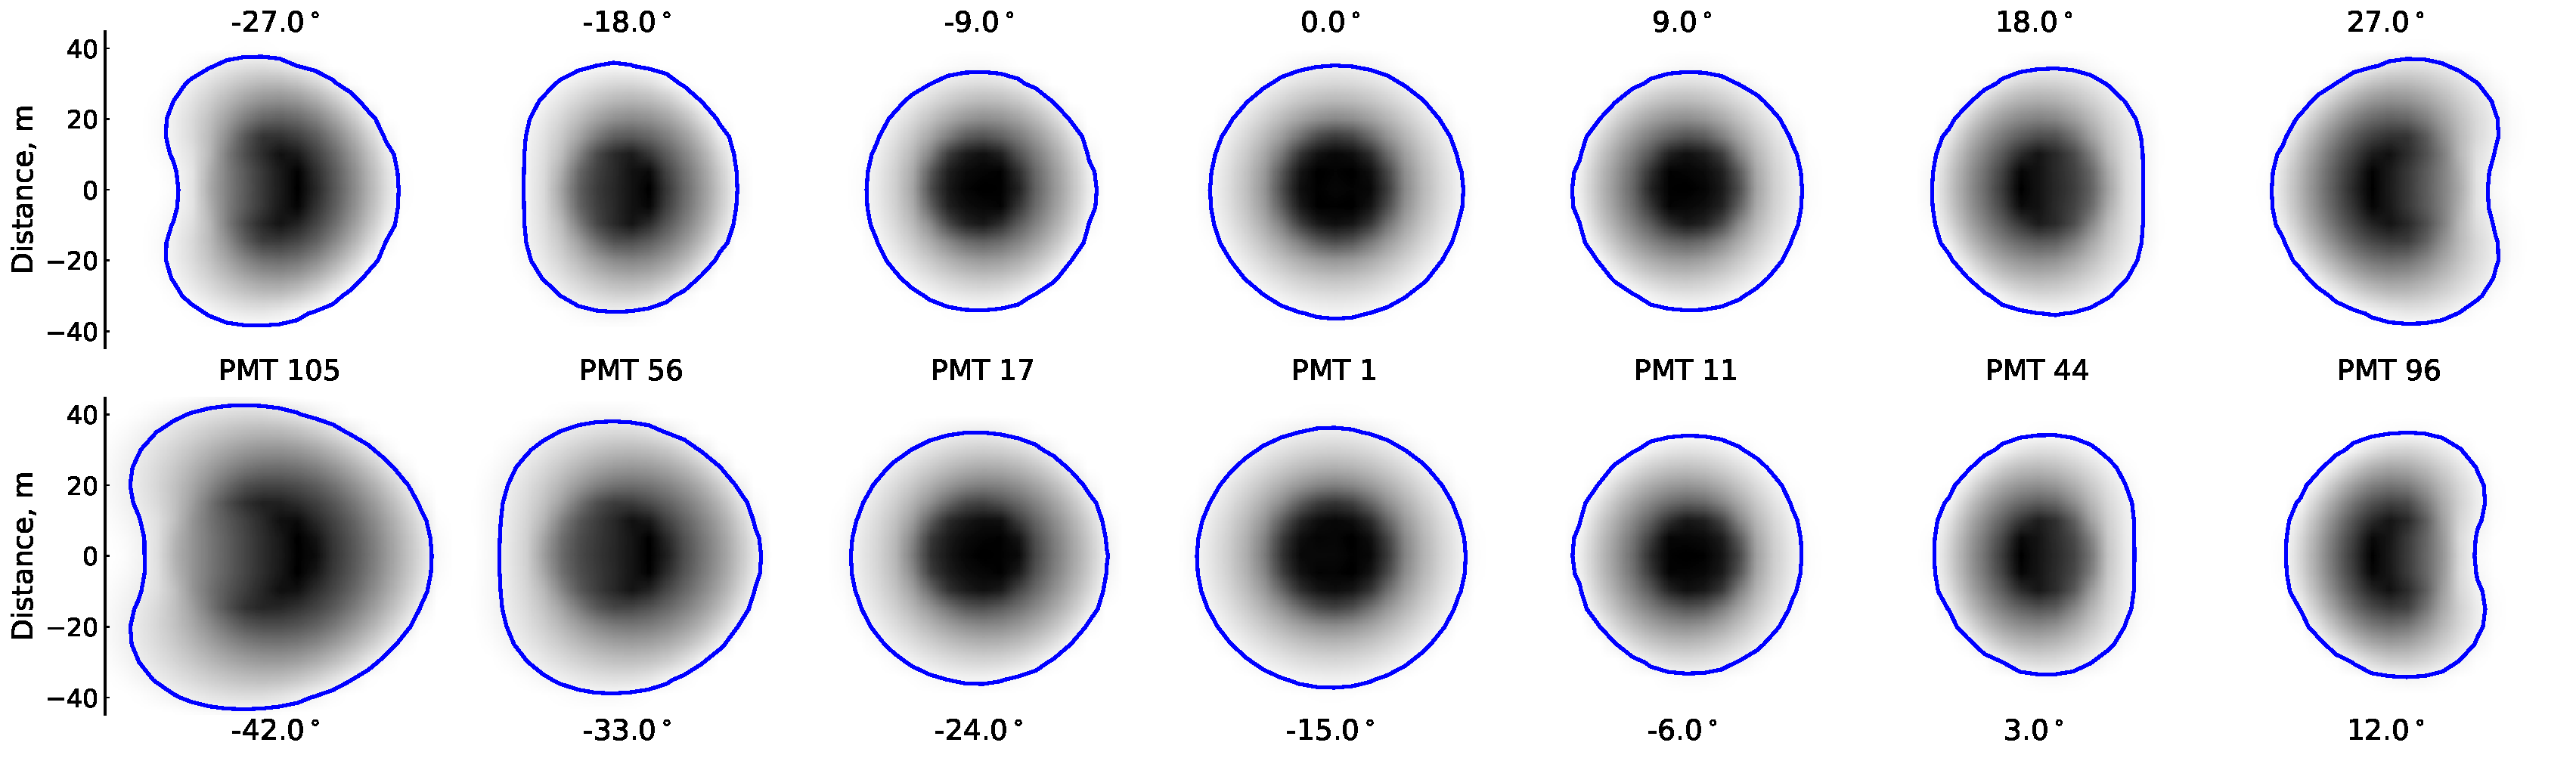
\includegraphics[width=0.95\textwidth]{figs/fov_inclined.pdf}
%    %\vspace{10pt}
%    %\includegraphics[width=0.49\textwidth]{fov_log.eps}%
%    \caption{The PMT FOVs at altitude $H=$ 1000~m. In top row presented are FOVs for PMTs No 1, 5, 14, 29, 50 and 77 that form a row across the mosaic (see Fig.~\ref{fig:2012-3_shore_image}) in assumption of vertical detector optical axis position. The bottom row shows same PMTs by for the inclined detector. The change in PMT FOVs is evident. The central PMT in the calculations is the Hamamatsu R3886 that has 35 mm photocathode and thus a larger FOV than FEU 84-3 PMTs used on other positions in the detector.}
%\label{fig:pmt_fov}
%\end{figure*}

\section{Conclusions \label{sect:conclusions}}
The SPHERE-2 detector operational 2008--2013 had a large array of supplementary sensor that allowed control and subsequent reconstruction of detector state and measurements conditions. 

The vital for reflected CL method information on detector position and orientation measured with good precision and reliability and were cross-checked using experimental data.
Measurements of the air pressure and temperature during flights gave information on the atmosphere state that in advance will allow to introduce different atmospheric models into analysis and to account of their impact on the results.

  
%{В статье представлена наиболее полная информация о номенклатуре и характеристиках всех датчиков  использованных в эксперименте с установкой СФЕРА-2. Описано назначение каждого датчика и частота (период) опроса (чтения) данных. Результаты измерений были использованы для учёта влияния условий окружающей среды при регистрации отражённого ЧС ШАЛ, а также при восстановлении характеристик ШАЛ от ПКЛ (не в этой статье).
%Основными факторами влияния являются высота, положение и наклон установки. Кроме того, заметное влияние оказывает уровень звездного фона оцениваемое по значению постоянного тока в каждом канале. Исследовано и учтено расхождение в данных о высоте с GPS приёмника и барометрического высотомера. Обнаружено скачкообразное изменение плотности атмосферы из-за погодных аномалий которое может приводить к заметной систематической ошибке при оценке состава ПКЛ. В работе были проанализированы и обобщены все зарегистрированные изменения условий окружающей среды и модификации аппаратуры за несколько лет измерений для уточнения и унификации результатов.

%В статье мы описали как в эксперименте мы измеряем параметры установки  СФЕРА-2, важные для восстановления черенковских событий.  В частности, высота установки над уровнем земли измеряется двумя способами, что позволяет определить истинное значение высоты. Мы видим, что установка стабильна в воздушном потоке.}

%\todoi{ВЫВОДЫ!!!!!!!! Их нет!!!!!} % сделано 2021/01/20

\section{Acknowledgments}
%done
We are grateful to the Lebedev Physical Institute of Russian Academy of Sciences group (leader S.B.~Shaulov) for assistance in assembling and testing the electronic equipment and in preparation of expeditions. We also thank the Baikal-GVD collaboration and G.V.~Domogatsky (Institute for Nuclear Research, Russian Academy of Sciences) for the support of the SPHERE experiment at the Baikal Lake scientific station.

%%%%%%%%%%%%%%%%%%%%%%%%%%%%%%%%%%%%%%%%%%%%%%%%%%%%%%%%%%%%%%%%%%%%%%%%

%\section{References}
\bibliography{Sphere-Data.bib}

\end{document}